% PP-Article.tex for AEA last revised 22 June 2011
%\documentclass[draftmode]{AEA}
\documentclass[AER]{AEA}

%\documentclass[12pt, a4paper]{article}
% If you have trouble with the mathtime package please see our technical support 
% document at: http://www.aeaweb.org/templates/technical_support.pdf
% You may remove the mathtime package if you can't get it working but your page
% count may be inaccurate as a result.
%\usepackage[cmbold]{mathtime}

% Note: you may use either harvard or natbib (but not both) to provide a wider
% variety of citation commands than latex supports natively. See below.

% Uncomment the next line to use the natbib package with bibtex 
\usepackage{natbib}

% Uncomment the next line to use the harvard package with bibtex
%\usepackage[abbr]{harvard}

%other packages
\usepackage{booktabs} % Allows the use of \toprule, \midrule and \bottomrule in tables
\usepackage{comment}
\usepackage{xcolor}
\usepackage{hyperref}
\usepackage{amsmath,amssymb,amsthm}
\usepackage{graphicx} % Allows including images
\usepackage{multicol}
\usepackage{multirow}
\usepackage{forest}
\usepackage{lscape}
\usepackage{adjustbox}
\usepackage{multicol}
\setlength{\columnsep}{1cm}
\usepackage{pgf,tikz}
\usepackage{subcaption} %for subfigure
%\usepackage{float} %For better positioning of objects
\forestset{qtree/.style={for tree={parent anchor=south, 
           child anchor=north,align=center,inner sep=0pt}}}

\usepackage{progressbar}

\usepackage{csquotes}
\usepackage{setspace}
           

%For number in equations with 'align'
\newcommand{\tabnotes}[2]{\bottomrule \multicolumn{#1}{@{}p{0.70\linewidth}@{}}{\footnotesize #2 }\end{tabular}\end{table}}

\newcommand\numberthis{\addtocounter{equation}{1}\tag{\theequation}} %https://tex.stackexchange.com/questions/42726/align-but-show-one-equation-number-at-the-end


%For quotting we define this 2:
\SetBlockThreshold{2}
\newcommand\myblockquote[2]{%
  \blockquote{\hspace*{2em}\emph{`#1'}\hfill(#2)}\par}


%For links
\definecolor{darkblue}{rgb}{0.0, 0.0, 0.65}
\definecolor{darkgreen}{rgb}{0.0, 0.65, 0.0}
\hypersetup{
	citecolor=blue,
	colorlinks=true,
	linkcolor=blue,
	filecolor=magenta,
	urlcolor=magenta
}

\let\footnote\thanks
%Prevent Footnote from breaking pages
\interfootnotelinepenalty=10000

%\usepackage[round]{natbib}


% This command determines the leading (vertical space between lines) in draft mode
% with 1.5 corresponding to "double" spacing.
\draftSpacing{1.5}

\begin{document}

%Has information on all the statistics estimated
\input{./macros.tex} 

%Full text

\title{When the Household Becomes the School: Sibling Effects on Parental Attention and Educational Outcomes During School Closures} %Sibling Spillovers from College Admission: Impacts on School Performance and Parental Expectations
\shortTitle{School closures and family size}
\author{
	Francisco Pardo \\
    \textit{\textcolor{red}{Preliminary Draft: Do Not Circulate}}
    %\textbf{University of Texas at Austin \footnote{\textit{Address:} 2908 Pearl Street APT C, Austin, Texas, 78705. \textit{phone:} +1 (202) 412-3049. \textit{email:} fpardo\@utexas.edu. \textit{webpage:} francisco-pardo-pajuelo.github.io.}}
	%\and
    %Author 2 \\
    %\textbf{Institution 2}
}
\date{\today}
%\pubMonth{}
%\pubYear{}
%\pubVolume{}
%\pubIssue{}
\JEL{}
\Keywords{}
%
\begin{abstract}


\\
\textit{JEL Codes: I21, I24}
\end{abstract}

%   I2 Education and Research Institutions
    % 	I20 	General 
    %   I21 	Analysis of Education
    %	I23 	Higher Education • Research Institutions
    %	I24 	Education and Inequality
    %	I26 	Returns to Education 
    %   I28 	Government Policy     
    
%   D1 	Household Behavior and Family Economics 
    % 	D13 	Household Production and Intrahousehold Allocation 
    %   D19  other

%   J2 	Demand and Supply of Labor 
    %   J24 	Human Capital • Skills • Occupational Choice • Labor Productivity 

%   O1 	Economic Development 
    %   O15 	Human Resources • Human Development • Income Distribution • Migration 

%   R2 	Household Analysis  
    % 	R23 	Regional Migration • Regional Labor Markets • Population • Neighborhood Characteristics 






\maketitle

%\newpage

%\begin{multicols}{2}
%
%%%%%%%%%%%%%%%%%%%%%%%%%%%%%%%%%%%%%%%%%%%%%%%%%%%%%%
%YOU HAVE ALREADY MADE A BACKUP. EDIT THIS FREELY
%%%%%%%%%%%%%%%%%%%%%%%%%%%%%%%%%%%%%%%%%%%%%%%%%%%%%%


\textbf{Research Question:} \textcolor{blue}{\textbf{`Do older siblings college experience affect their younger siblings aspirations, effort and actions over higher education?'}}


\textbf{Literature}
\begin{itemize}
    \item  Effects are strong on the choices they make, mainly following their older siblings to the same college. Less clear results on overall applications and enrollment. Null results on effort during high school.
    \item Some evidence of stronger effects when siblings are more similar (in age or sex). Mixed results and no clarity on mechanisms. \footnote{}\footnotetext{\cite{dustan_family_2018}, \cite{joensen_spillovers_2018}, \cite{altmejd_o_2021}, \cite{aguirre_walking_2021}, \cite{de_gendre_class_2021}, \cite{avdeev_spillovers_2024}, \cite{dahl_intergenerational_2024}}
\end{itemize}

\textbf{Motivation:}
\begin{itemize}
    \item Peru has decentralized applications and exams. This contrasts with systems like Chile, where there is a centralized application system (choice set) with a standardized exam for all applications. This creates bigger information barriers and costs for applications that may cause larger spillover effects. It also creates methodological challenges that a centralized system does not.
    \item I have school administrative data with exams in 2nd, 4th and 8th grade and survey data to students and parents on behavior, beliefs, expectations, etc. This allows for unexplored effects in early childhood and in mechanisms. In terms of outcomes, we can explore: 8th grade student's aspirations of going to college, 8th grade exams (earlier than literature) and full school grade progression.
\end{itemize}

\textbf{Strategy:} I do fuzzy regression discontinuity using college-major-semester (cell) cutoffs. (i) I estimate the likely cutoff for each cell, (ii) stack all applications, (iii) estimate an RD model with cell fixed effects. This is done with for the oldest sibling, with effects estimated on their younger siblings (after the application). This is done for all public universities in the country from 2017-2023.

\textbf{Results:}
     The first stage is quite big. Being above the cutoff means a 70\% increased chance of admission and 50\% of enrollment to the applied cutoff. Being above the cutoff also increases enrollment in ANY university EVER by 18\%. \hyperref[fig:first_stage]{Figure \ref{fig:first_stage}}. Results for the full sample are as follow:

\begin{itemize}    
    \item College choices: \hyperref[tab:table_sib_choices_all_1_2]{Table \ref{tab:table_sib_choices_all_1_2}}
    \item School progression:  \hyperref[tab:table_sib_school_outcomes_all_1_2]{Table \ref{tab:table_sib_school_outcomes_all_1_2}}
    \item College aspirations: \hyperref[tab:table_sib_univ_outcomes_all_1_2]{Table \ref{tab:table_sib_univ_outcomes_all_1_2}}
    \item Heterogeneous analysis: \hyperref[tab:table_sib_heterog_all_1_2]{Table \ref{tab:table_sib_heterog_all_1_2}}
    \item Balance test: \hyperref[tab:table_foc_balance_all_1_2]{Table \ref{tab:table_foc_balance_all_1_2}}
\end{itemize}    

\begin{itemize}  
    \item When restricting only for the first semester each focal child applies results look stronger but possibly caused by unbalanced sample: \hyperref[tab:table_sib_choices_first_1_2]{Table \ref{tab:table_sib_choices_first_1_2}}, \hyperref[tab:table_sib_school_outcomes_first_1_2]{Table \ref{tab:table_sib_school_outcomes_first_1_2}}, \hyperref[tab:table_sib_univ_outcomes_first_1_2]{Table \ref{tab:table_sib_univ_outcomes_first_1_2}}, \hyperref[tab:table_sib_heterog_first_1_2]{Table \ref{tab:table_sib_heterog_first_1_2}}, \hyperref[tab:table_foc_balance_first_1_2]{Table \ref{tab:table_foc_balance_first_1_2}}.
\end{itemize}   

\newpage
\textbf{Issues:}
\begin{itemize}
    \item In centralized settings, it is common to keep the first set of choices/application. It is not clear I can do the same here since I don't (currently) have dates of exams, but even then, that would mean only keep 1 exam.
    \item I am considering 2 options: Use full sample and use only first semester of applications. I also considered using only those who apply once but sample is too small.
    \item I am not sure if using the full sample is methodologically correct, although it seems balanced. Results there however look very similar to \cite{altmejd_o_2021} in the case of choices.
    \item Main problem now is the balance is not working properly for 8th grade exams when keeping only the first semester.
\end{itemize}



%\section{Introduction}
%\label{sec:intro}


%\footnote{}\footnotetext{example footnote}

%medication/treatment  (\cite{sokol_impact_2005})
%\section{Literature review and contribution}
%\label{sec:literature}


%\section{Context}
%\label{sec:context}


%\section{Data}
%\label{sec:data}

%\section{Empirical Strategy}
%\label{sec:empirical}


%General RD
%\begin{align*}
%Y_{it}=\alpha_{i} + \beta {ABOVE} + \gamma  f(Age) + \delta X_{it} + \epsilon_{it} \numberthis \label{eq_main}
%\end{align*}



%\section{Mechanisms}
%\label{sec:mechanisms}


%\section{Heterogenity}
%\label{sec:heterogeneity}

%\section{Conclusion}
%\label{sec:conclusion}

%\subsection{Future Research}
%\label{sec:future}



%%%%%%%%%%%%%%%%%%%%%%%%%%%%%%%%%%%%%%
% Figures and Tables 
%%%%%%%%%%%%%%%%%%%%%%%%%%%%%%%%%%%%%%

%:::::::::::::: FIGURES


%\input{./figures/figure1.tex} 


%\clearpage

%:::::::::::::: TABLES


%\input{./tables/mechanisms.tex}




%%%%%%%%%%%%%%
% Introduction
%%%%%%%%%%%%%%

% 1. Motivation (1 Pargraph)


% Learning losses from school closures
%During the COVID-19 pandemic and school closures, many countries implemented some form of remote learning. Suddenly without the usual school inputs,  parents had a bigger role in the education of their children. This period caused significant learning losses, especially for more vulnerable populations (\cite{haelermans_inequality_2022}, \cite{jakubowski_global_2023}). Yet, with parents as a more relevant input in the education production function and remote schooling that required digital resources, there is no evidence on how the size of the household could have affected children's learning.


% Siblings did much worse (PISA score)

% Questions about family size being relevant?


% 2. Research question


% 6. Roadmap of paper.
The paper proceeds as follows. \hyperref[sec:empirical_strategy]{Section \ref{sec:empirical_strategy}} details the empirical approach. \hyperref[sec:data]{Section \ref{sec:data}}  describes the higher education system in Peru and linked administrative data. \hyperref[sec:results]{Section \ref{sec:results}} presents results. \hyperref[sec:mechanisms]{Section \ref{sec:mechanisms}} discusses potential mechanisms. \hyperref[sec:heterogeneity]{Section \ref{sec:heterogeneity}} discusses heterogeneity in results. \hyperref[sec:robustness]{Section \ref{sec:robustness}} shows robustness checks. \hyperref[sec:policy]{Section \ref{sec:policy}} discusses policy implications. \hyperref[sec:conclusions]{Section \ref{sec:conclusions}} concludes.

\hyperref[fig:pisa]{Figure \ref{fig:pisa}}

\hyperref[fig:fig2]{Figure \ref{fig:fig2}}


\hyperref[tab:twfe_ece]{Table \ref{tab:twfe_ece}}

\hyperref[tab:twfe_ece_survey_1]{Table \ref{tab:twfe_ece_survey_1}}

\hyperref[tab:twfe_ece_survey_2]{Table \ref{tab:twfe_ece_survey_2}}

\hyperref[tab:rd_ece_index_365]{Table \ref{tab:rd_ece_index_365}}

\hyperref[tab:rd_summ_K_m_a_365]{Table \ref{tab:rd_summ_K_m_a_365}}

\hyperref[tab:rd_summ_2_m_a_365]{Table \ref{tab:rd_summ_2_m_a_365}}


%%%%%%%%%%%%%%
% Empirical Strategy
%%%%%%%%%%%%%%

\section{Empirical Strategy}\label{sec:empirical_strategy}

Main identification


Validation 


%%%%%%%%%%%%%%
% Data
%%%%%%%%%%%%%%
\section{Data}\label{sec:data}

\subsection{SIAGIE}

\subsection{ECE}

\subsection{Sibling Identification}

%%%%%%%%%%%%%%
% Results
%%%%%%%%%%%%%%
\section{Results}\label{sec:results}

\subsection{Learning Losses}

\subsubsection{GPA}

\subsubsection{Standardized Exams}

\subsection{Educational Trajectories}

\subsubsection{Grade Progression}

\subsubsection{Graduation and Higher Education}

\subsection{Expectations over educational attainment}

Using ECE survey from before and after covid we perform simple TWFE estimations. In \textcolor{green}{Table...} we see a reduction in parental expectations for attaining a 4-year college degree and an increase of those who believe the maximum level of education will be high-school.


%%%%%%%%%%%%%%
% Robustness and Mechanisms
%%%%%%%%%%%%%%
\section{Mechanisms}\label{sec:mechanisms}

Them main potential mechanisms are...

\subsection{Birth Order}

Results hold when working only with first births

\subsection{Socio economic and human capital constraints in the household}

Results hold when controlling for level of education, internet and pc.

We also look into the number of rooms

\subsection{Sibling disruptions}

Results hold when doing age gap.

\subsection{Parental time and investment}

Results by single/both parents. Other adults in the household.

Results from RD of SSA

Results from \hyperref[tab:rd_summ_1_m_a_365]{Table \ref{tab:rd_summ_1_m_a_365}} show how delaying school has a negative effect in the older sibling. \footenote{a}

\subsection{Income}

Results from socio-economic status show that... 
This is highly correlated with income... (show)
However, it is certainly not a malleable, but it is evidence that there is not differential loss in income driving the results.

Perhaps show that there are losses of socio-economic status overall? Can we do this with household surveys or with the ECE surveys themselves?

\section{Heterogeneity}\label{sec:heterogeneity}

Surprisingly, results are consistent across...

\subsection{Reinforcement vs Compensation}

\section{Robustness}\label{sec:robustness}

\subsection{Potential sample selection}

Discuss how siblings are observed. We only see observations as long as they are enrolled in data. Most children are enrolled in primary school \textcolor{green}{(show data from household surveys)}. However, most children are not enrolled until 3-4 years old. Since our last year of administrative data is 2024, this means that some families with 2 children, one of which was born after 2021, might be observed as only childs. To address any concerns from this selection I do the following:

\begin{itemize}
    \item These families are not particularly different from others? (this true)?
    \item I use data up to 2023 and 2022 to define families (and potentially imposing a similar bias to earlier years) and still see results change around COVID. \textcolor{green}{Pending Analyis}
\end{itemize}


\subsection{Siblings in same vs different schools}

\subsection{Different definitions of siblings: father, both, caretaker}

\subsection{Younger and middle child}

\subsection{Unadjusted scores}

%%%%%%%%%%%%%%
% Policy Discussion
%%%%%%%%%%%%%%
\section{Policy Discussion}\label{sec:policy}

%%%%%%%%%%%%%%
%Conclusions
%%%%%%%%%%%%%%
\section{Conclusions}\label{sec:conclusions}


%We argue that an older sibling’s enrollment in a higher quality college can provide for families information about postsecondary education that would otherwise be difficult or impossible to obtain. [draft US]





%\blindtext \blindtext
%\end{multicols}


\newpage
% Remove or comment out the next two lines if you are not using bibtex.
\bibliographystyle{aea}
\bibliography{references.bib}

\newpage

%First stage



\begin{figure}[htbp]
    \centering
    
    \begin{subfigure}{\textwidth}
        \centering
        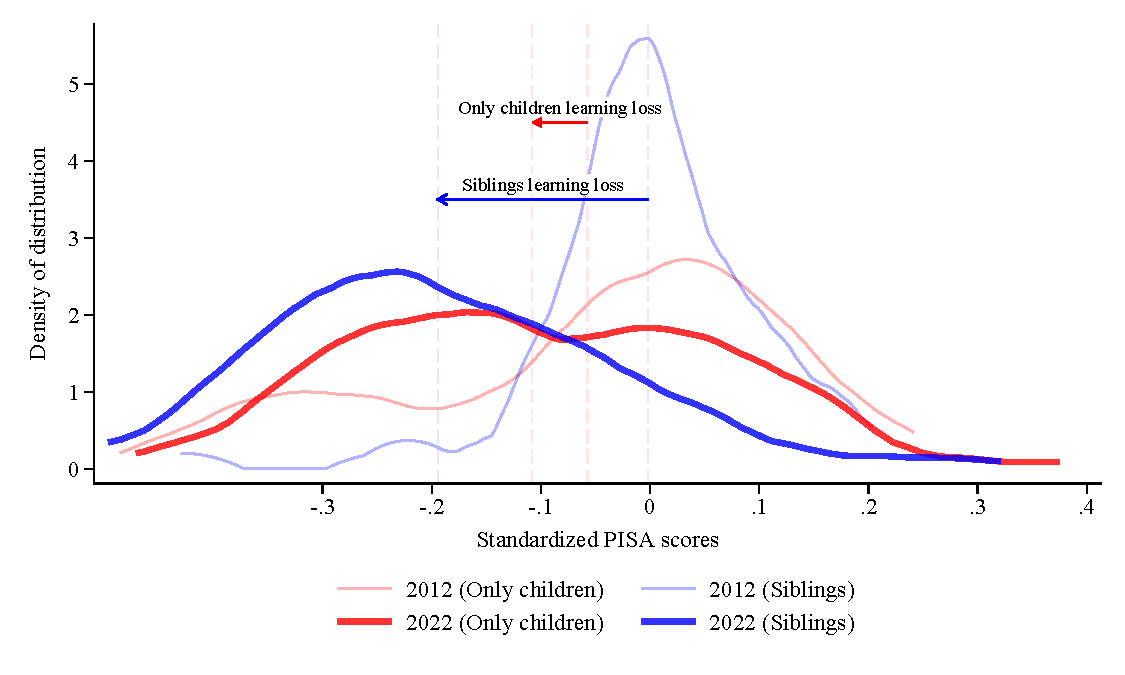
\includegraphics[width=\textwidth]{./FIGURES/Descriptive/PISA_distribution_2012_2022_PV4MATH.pdf}
        \caption{Learning gaps in Mathematics by year}
        \label{fig:1a}
    \end{subfigure}
    
    \vspace{1em} % Add some vertical space between subfigures
    
    \begin{subfigure}{\textwidth}
        \centering
        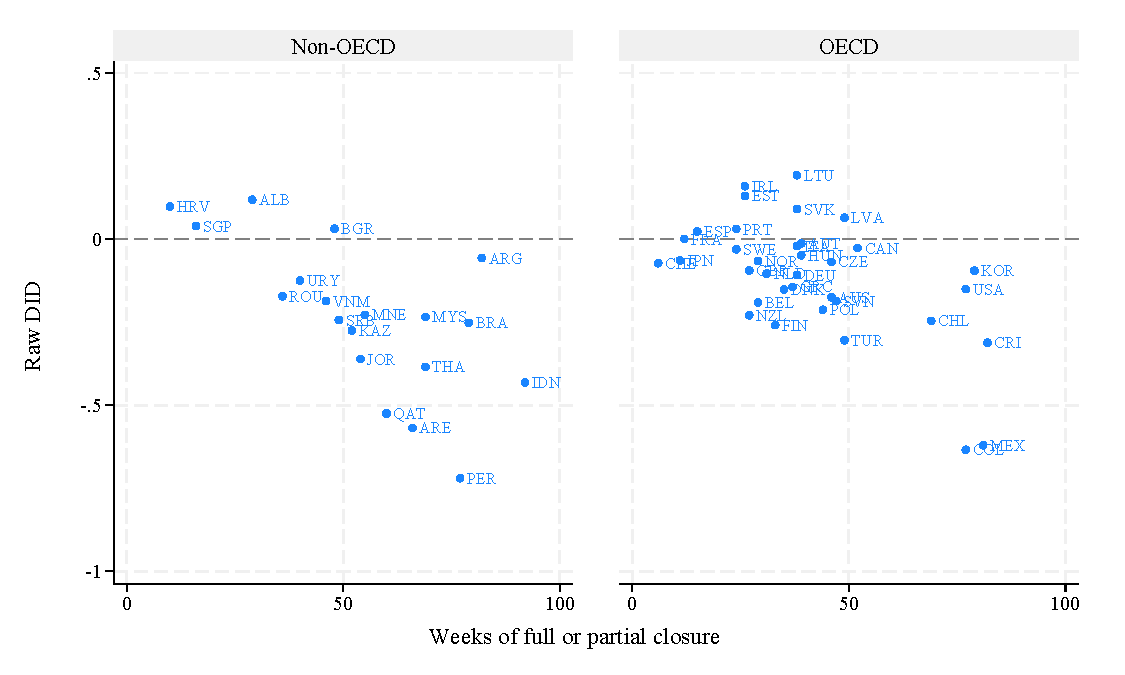
\includegraphics[width=\textwidth]{./FIGURES/Descriptive/PISA_raw_DID_PV4MATH_not_fully_open.pdf}
        \caption{Change in learning gaps by duration of school closure for OECD and Non-OECD countries.}
        \label{fig:1b}
    \end{subfigure}
    
    \caption{Learning gaps around the world}
    \label{fig:pisa}
\end{figure}



\begin{figure}[htbp]
    \centering
    
    \begin{subfigure}{\textwidth}
        \centering
        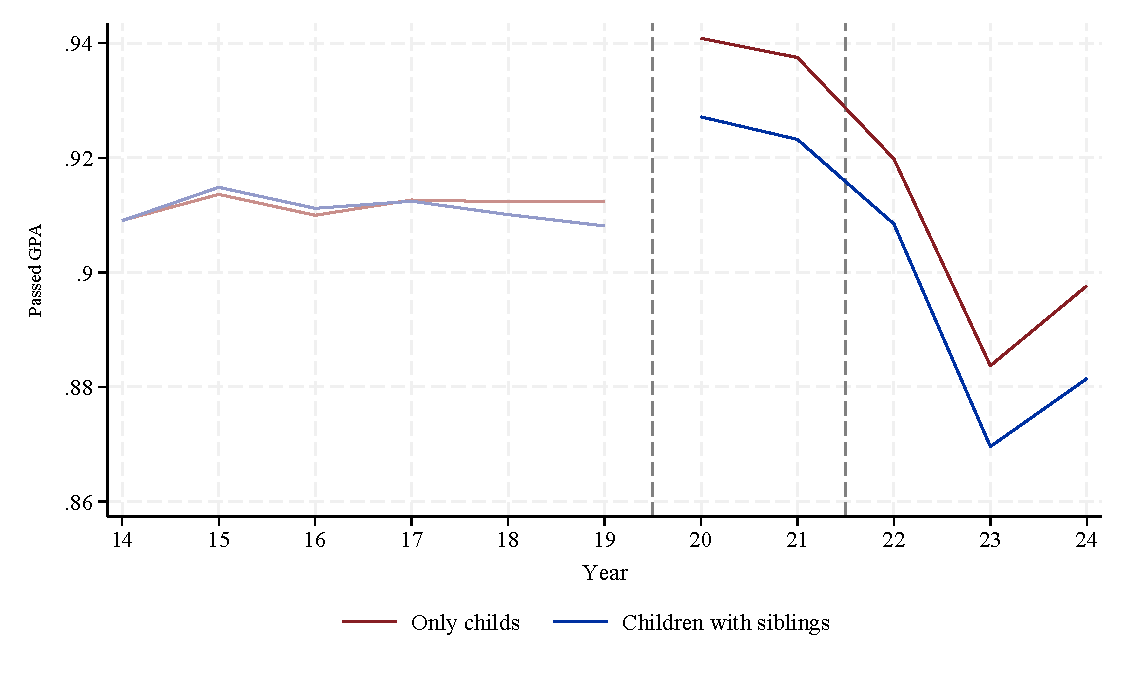
\includegraphics[width=\textwidth]{./FIGURES/Descriptive/raw_total_elm_pass_math_siblings.pdf}
        \caption{\% of students with a A in Mathematics from 1st-6th grade}
        \label{fig:trend_pass}
    \end{subfigure}
    
    \vspace{1em} % Add some vertical space between subfigures
    
    \begin{subfigure}{\textwidth}
        \centering
        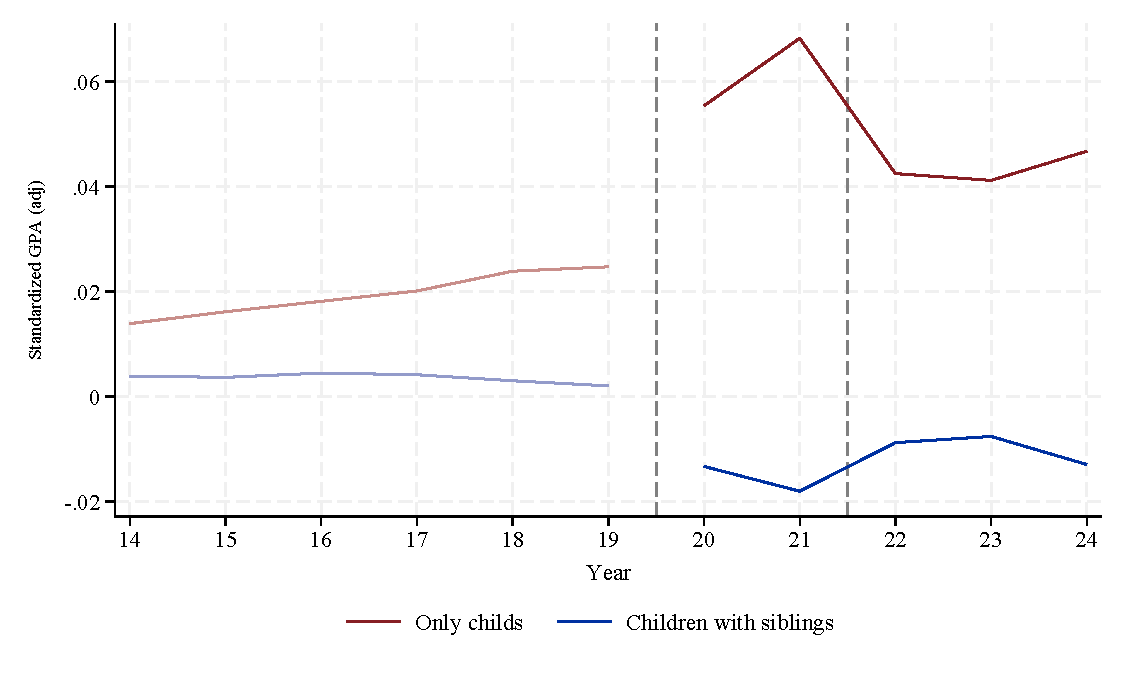
\includegraphics[width=\textwidth]{./FIGURES/Descriptive/raw_total_elm_std_gpa_m_adj_siblings.pdf}
        \caption{Average GPA standardized within school-grade-year from 1st-6th grade}
        \label{fig:trend_gpa}
    \end{subfigure}
    
    \caption{Trends in education outcomes for only children and children with siblings}
    \label{fig:trend}
\end{figure}


\begin{figure}[htbp]
    \centering
    
    \begin{subfigure}{\textwidth}
        \centering
        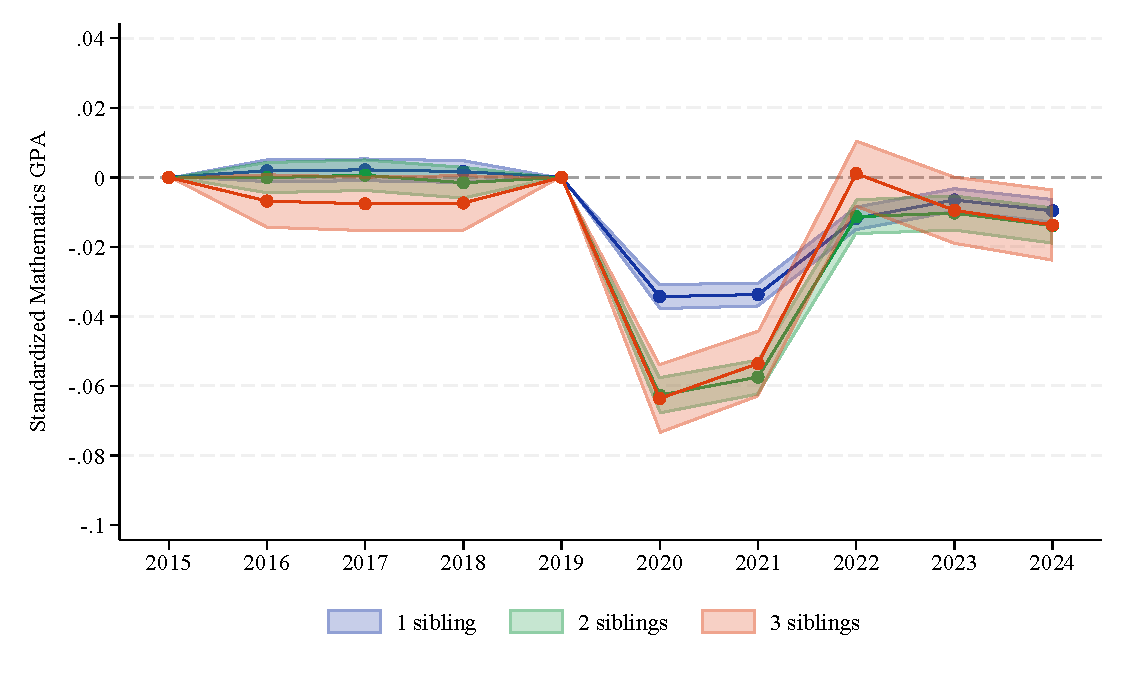
\includegraphics[width=\textwidth]{./FIGURES/Event Study/covid_event_bysibs_all_all_std_gpa_m_adj_Tsiblings_Soldest_4.pdf}
        \caption{Event Study}
        \label{fig:main_result_event}
    \end{subfigure}
    
    \vspace{1em} % Add some vertical space between subfigures
    
    \begin{subfigure}{\textwidth}
        \centering
        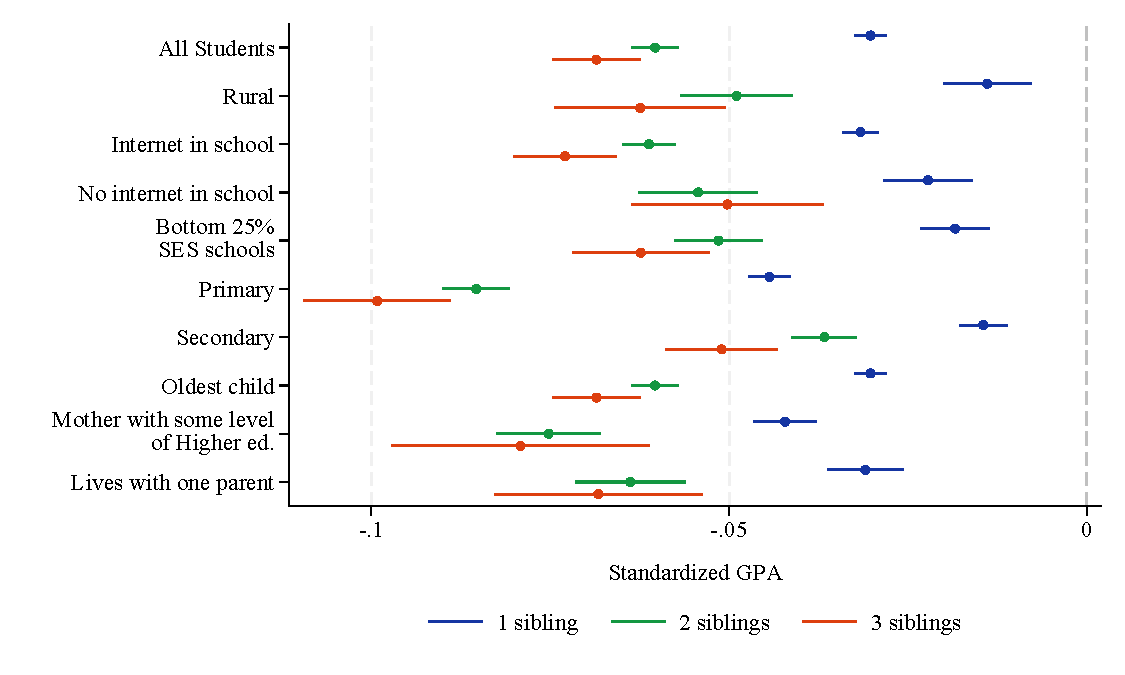
\includegraphics[width=\textwidth]{./FIGURES/TWFE/covid_twfe_summ_bysibs_all_20-21_gpa_m_adj_Tsiblings_Soldest_4.pdf}
        \caption{Change in gap between children with siblings and only childs}
        \label{fig:main_result_twfe}
    \end{subfigure}
    
    \caption{Learning gap between only childs and siblings}
    \label{fig:main_result}
\end{figure}


\clearpage

%RD-first grade
\makeatletter
\@ifclassloaded{beamer}{%
       \centering
       \resizebox{0.6\textwidth}{!}%
}{%
       \begin{table}[!tbp]\centering\def\sym#1{\ifmmode^{#1}\else\(^{#1}\)\fi}
       \centering
       \caption{TWFE on 8th grade GPA and standardized exams controlling for baseline 2nd grade standardized exams}
       \label{tab:twfe_ece}
       \resizebox{0.95\textwidth}{!}%
}
{
\makeatother
\begin{tabular}{lcccc}
\toprule
\cmidrule(lr){2-5}
& \multicolumn{4}{c}{TWFE} \\
\cmidrule(lr){2-5}
& 1-3 siblings & 1 sibling & 2 siblings & 3 siblings  \\
\cmidrule(lr){2-2} \cmidrule(lr){3-3} \cmidrule(lr){4-4} \cmidrule(lr){5-5}
& (1) & (2) & (3) & (4) \\
\bottomrule
&  &  & &  \\
&  &  & &  \\
\multicolumn{5}{l}{Panel A: GPA } \\
Mathematics         &      -0.099***&      -0.011   &      -0.036***&      -0.059***\\
                    &     (0.009)   &     (0.009)   &     (0.011)   &     (0.015)   \\
                    &               &               &               &               \\
Observations        &     326,669   &     279,833   &     225,092   &     179,575   \\
 
&  &  & &  \\
Reading             &      -0.099***&      -0.010   &      -0.031***&      -0.034** \\
                    &     (0.009)   &     (0.009)   &     (0.010)   &     (0.015)   \\
                    &               &               &               &               \\
Observations        &     326,669   &     280,846   &     225,840   &     180,218   \\
 
&  &  & &  \\
\multicolumn{5}{l}{Panel B: Standardized Exams } \\
Mathematics         &      -0.034***&      -0.017** &      -0.044***&      -0.071***\\
                    &     (0.006)   &     (0.007)   &     (0.008)   &     (0.011)   \\
                    &               &               &               &               \\
Observations        &     409,527   &     282,640   &     227,403   &     181,370   \\
 
&  &  & &  \\
Reading             &      -0.013** &       0.002   &      -0.022***&      -0.046***\\
                    &     (0.006)   &     (0.006)   &     (0.008)   &     (0.011)   \\
                    &               &               &               &               \\
Observations        &     409,690   &     282,769   &     227,486   &     181,466   \\
 

\bottomrule
\end{tabular}
}
\@ifclassloaded{beamer}{%
}{%
       \end{table}
}

\makeatletter
\@ifclassloaded{beamer}{%
       \centering
       \resizebox{0.6\textwidth}{!}%
}{%
       \begin{table}[!tbp]\centering\def\sym#1{\ifmmode^{#1}\else\(^{#1}\)\fi}
       \centering
       \caption{TWFE on GPA by baseline resources}
       \label{tab:twfe_gpa_baseline_survey_1_pairall}
       \resizebox{0.65\textwidth}{!}%
}
{
\makeatother
\begin{tabular}{lccc}
\toprule
\cmidrule(lr){2-4}
& \multicolumn{3}{c}{TWFE} \\
\cmidrule(lr){2-4}
& 1 sibling & 2 siblings & 3 siblings  \\
\cmidrule(lr){2-2} \cmidrule(lr){3-3} \cmidrule(lr){4-4}
& (1) & (2) & (3)\\
\bottomrule
&  &  &  \\
&  &  &   \\
\multicolumn{4}{l}{\textit{Panel A: All studentes}} \\
\hspace{3mm}Mathematics&      -0.028***&      -0.061***&      -0.080***\\
                    &     (0.004)   &     (0.005)   &     (0.009)   \\
 
%&  &  &   \\
\hspace{3mm}Reading &      -0.018***&      -0.044***&      -0.052***\\
                    &     (0.004)   &     (0.005)   &     (0.009)   \\
                    &               &               &               \\
\hspace{3mm}Observations&   1,285,073   &   1,038,874   &     906,608   \\
 
&  &  &   \\
\multicolumn{4}{l}{\textit{Panel B: Low SES Households (Q1)}} \\
\hspace{3mm}Mathematics&      -0.009   &      -0.028***&      -0.061***\\
                    &     (0.007)   &     (0.009)   &     (0.014)   \\
 
%&  &  &   \\
\hspace{3mm}Reading &      -0.003   &      -0.016*  &      -0.040***\\
                    &     (0.007)   &     (0.009)   &     (0.014)   \\
                    &               &               &               \\
\hspace{3mm}Observations&     312,464   &     264,200   &     226,444   \\
 
&  &  &   \\
\multicolumn{4}{l}{\textit{Panel C: High SES Households (Q4)}} \\
\hspace{3mm}Mathematics&      -0.037***&      -0.065***&      -0.113***\\
                    &     (0.008)   &     (0.014)   &     (0.034)   \\
 
%&  &  &   \\
\hspace{3mm}Reading &      -0.029***&      -0.070***&      -0.017   \\
                    &     (0.008)   &     (0.014)   &     (0.034)   \\
                    &               &               &               \\
\hspace{3mm}Observations&     257,212   &     199,735   &     179,355   \\
 
&  &  &   \\
\multicolumn{4}{l}{\textit{Panel D: Households with no PC or Internet}} \\
\hspace{3mm}Mathematics&      -0.032***&      -0.079***&      -0.067***\\
                    &     (0.006)   &     (0.009)   &     (0.019)   \\
 
%&  &  &   \\
\hspace{3mm}Reading &      -0.023***&      -0.056***&      -0.051***\\
                    &     (0.006)   &     (0.009)   &     (0.019)   \\
                    &               &               &               \\
\hspace{3mm}Observations&     454,966   &     366,342   &     320,367   \\
 
&  &  &   \\
\multicolumn{4}{l}{\textit{Panel E: Households with both PC and Internet}} \\
\hspace{3mm}Mathematics&      -0.023***&      -0.035***&      -0.098***\\
                    &     (0.006)   &     (0.009)   &     (0.015)   \\
 
%&  &  &   \\
\hspace{3mm}Reading &      -0.008   &      -0.039***&      -0.061***\\
                    &     (0.006)   &     (0.009)   &     (0.015)   \\
                    &               &               &               \\
\hspace{3mm}Observations&     438,221   &     355,035   &     307,508   \\
 

\bottomrule
\end{tabular}
}
\@ifclassloaded{beamer}{%
}{%
       \end{table}
}

\makeatletter
\@ifclassloaded{beamer}{%
       \centering
       \resizebox{0.6\textwidth}{!}%
}{%
       \begin{table}[!tbp]\centering\def\sym#1{\ifmmode^{#1}\else\(^{#1}\)\fi}
       \centering
       \caption{WFE on GPA by baseline achievement and expectations}
       \label{tab:twfe_gpa_baseline_survey_2_pairall}
       \resizebox{0.65\textwidth}{!}%
}
{
\makeatother
\begin{tabular}{lccc}
\toprule
\cmidrule(lr){2-4}
& \multicolumn{3}{c}{TWFE} \\
\cmidrule(lr){2-4}
& 1 sibling & 2 siblings & 3 siblings  \\
\cmidrule(lr){2-2} \cmidrule(lr){3-3} \cmidrule(lr){4-4}
& (1) & (2) & (3)\\
\bottomrule
&  &  &  \\
&  &  &   \\
\multicolumn{4}{l}{\textit{Panel A: All studentes}} \\
\hspace{3mm}Mathematics&      -0.028***&      -0.061***&      -0.080***\\
                    &     (0.004)   &     (0.005)   &     (0.009)   \\
 
%&  &  &   \\
\hspace{3mm}Reading &      -0.018***&      -0.044***&      -0.052***\\
                    &     (0.004)   &     (0.005)   &     (0.009)   \\
                    &               &               &               \\
\hspace{3mm}Observations&   1,285,073   &   1,038,874   &     906,608   \\
 
&  &  &   \\
\multicolumn{4}{l}{\textit{Panel B: Student in bottom quartile of achievement}} \\
\hspace{3mm}Mathematics&       0.001   &      -0.042***&      -0.106***\\
                    &     (0.007)   &     (0.010)   &     (0.015)   \\
 
%&  &  &   \\
\hspace{3mm}Reading &       0.009   &      -0.036***&      -0.064***\\
                    &     (0.008)   &     (0.010)   &     (0.016)   \\
                    &               &               &               \\
\hspace{3mm}Observations&     261,349   &     220,666   &     193,655   \\
 
&  &  &   \\
\multicolumn{4}{l}{\textit{Panel C: Student in top quartile of achievement}} \\
\hspace{3mm}Mathematics&      -0.045***&      -0.101***&      -0.140***\\
                    &     (0.007)   &     (0.011)   &     (0.023)   \\
 
%&  &  &   \\
\hspace{3mm}Reading &      -0.032***&      -0.069***&      -0.090***\\
                    &     (0.007)   &     (0.011)   &     (0.023)   \\
                    &               &               &               \\
\hspace{3mm}Observations&     364,927   &     282,401   &     245,220   \\
 
&  &  &   \\
\multicolumn{4}{l}{\textit{Panel D: Max Expectation: Finish school}} \\
\hspace{3mm}Mathematics&      -0.003   &      -0.030   &      -0.054*  \\
                    &     (0.014)   &     (0.019)   &     (0.030)   \\
 
%&  &  &   \\
\hspace{3mm}Reading &      -0.027*  &      -0.031   &      -0.059*  \\
                    &     (0.015)   &     (0.019)   &     (0.031)   \\
                    &               &               &               \\
\hspace{3mm}Observations&      84,652   &      71,387   &      61,974   \\
 
&  &  &   \\
\multicolumn{4}{l}{\textit{Panel E: Max Expectation: 4-year college or grad school}} \\
\hspace{3mm}Mathematics&      -0.033***&      -0.067***&      -0.095***\\
                    &     (0.004)   &     (0.006)   &     (0.011)   \\
 
%&  &  &   \\
\hspace{3mm}Reading &      -0.022***&      -0.049***&      -0.073***\\
                    &     (0.004)   &     (0.006)   &     (0.011)   \\
                    &               &               &               \\
\hspace{3mm}Observations&   1,039,027   &     830,658   &     724,846   \\
 

\bottomrule
\end{tabular}
}
\@ifclassloaded{beamer}{%
}{%
       \end{table}
}



\clearpage
\makeatletter
\@ifclassloaded{beamer}{%
       \centering
       \resizebox{0.6\textwidth}{!}%
}{%
       \begin{table}[!tbp]\centering\def\sym#1{\ifmmode^{#1}\else\(^{#1}\)\fi}
       \centering
       \caption{Effects of younger sibling delaying school on older sibling standardized exams - 1 - m - a -  - 365}
       \label{tab:rd_summ_1_m_a_365}
       \resizebox{0.95\textwidth}{!}%
}
{
\makeatother
\resizebox{\textwidth}{!}{
\begin{tabular}{lccc}
\toprule
\cmidrule(lr){2-4}
& \multicolumn{3}{c}{Standardized GPA} \\
\cmidrule(lr){2-4}
& Pre-Covid & Covid & Post-Covid  \\
& 2018-2019 & 2020-2021 & 2022-2023  \\
\cmidrule(lr){2-2} \cmidrule(lr){3-3} \cmidrule(lr){4-4}
& (1) & (2) & (3)  \\
\bottomrule
&  &  &   \\
\multirow{2}{*}{\shortstack[l]{Younger sibling born after \\ school-entry cutoff}}&      -0.023***&      -0.001   &      -0.023***\\
                    &     (0.007)   &     (0.007)   &     (0.006)   \\
Local Linear        &         Yes   &         Yes   &         Yes   \\
                    &               &               &               \\
Observations        &     358,861   &     354,044   &     447,536   \\
Counterfactual mean &       0.058   &       0.020   &       0.050   \\
Bandwidth           &         365   &         365   &         365   \\
 

\bottomrule
\end{tabular}
}
\@ifclassloaded{beamer}{%
}{%
       \end{table}
}

\makeatletter
\@ifclassloaded{beamer}{%
       \centering
       \resizebox{0.6\textwidth}{!}%
}{%
       \begin{table}[!tbp]\centering\def\sym#1{\ifmmode^{#1}\else\(^{#1}\)\fi}
       \centering
       \caption{Effects of younger sibling delaying school on older sibling standardized exams and parental investment}
       \label{tab:rd_ece_index_365}
       \resizebox{0.95\textwidth}{!}%
}
{
\makeatother
\begin{tabular}{lccccc}
\toprule
& \multicolumn{2}{c}{Pre-Covid}  & \multicolumn{3}{c}{Post-Covid} \\
& \multicolumn{2}{c}{2018-2019}  & \multicolumn{3}{c}{2022-2024}  \\
\cmidrule(lr){2-3} \cmidrule(lr){4-6}
& Mathematics & Reading & Mathematics & Reading & Parental Investment  \\
& (1) & (2) & (3) & (4) & (5) \\
\bottomrule
&  &  &  & &  \\
\multirow{2}{*}{\shortstack[l]{Younger sibling born after \\ school-entry cutoff}}&      -0.025*  &      -0.023*  &      -0.009   &      -0.012   &      -0.035***\\
                    &     (0.014)   &     (0.012)   &     (0.013)   &     (0.010)   &     (0.013)   \\
Local Linear        &         Yes   &         Yes   &         Yes   &         Yes   &         Yes   \\
                    &               &               &               &               &               \\
Observations        &      86,605   &      86,602   &     104,983   &     105,064   &     101,766   \\
Counterfactual mean &      -0.105   &      -0.083   &       0.194   &       0.288   &      -0.004   \\
Bandwidth           &         365   &         365   &         365   &         365   &         365   \\
 

\bottomrule
\end{tabular}
}
\@ifclassloaded{beamer}{%
}{%
       \end{table}
}








\clearpage
%\newpage

\setcounter{figure}{0}
\renewcommand\thefigure{A.\arabic{figure}}    

\setcounter{table}{0}
\renewcommand{\thetable}{A.\arabic{table}}


\begin{center}
\huge
\textbf{Appendix: NOT FOR PUBLICATION}
\normalsize
\end{center}


\section*{Appendix A: Robustness} \label{sec:appa}
\newpage


\makebox[0.1\width][l]{
\resizebox{\textwidth}{!}{
\begin{tabular}{lccc}
\toprule
\cmidrule(lr){2-4}
& \multicolumn{3}{c}{Standardized GPA}
\cmidrule(lr){2-4}
& Pre-Covid & Covid & Post-Covid  \\
& 2018-2019 & 2020-2021 & 2022-2023  \\
\cmidrule(lr){2-2} \cmidrule(lr){3-3} \cmidrule(lr){4-4}
& (1) & (2) & (3)  \\
\bottomrule
&  &  &   \\
Delay School (After SSA)&      -0.001   &      -0.010   &      -0.004   \\
                    &     (0.006)   &     (0.006)   &     (0.006)   \\
Local Linear        &         Yes   &         Yes   &         Yes   \\
                    &               &               &               \\
Observations        &     418,987   &     371,966   &     485,601   \\
Counterfactual mean &       0.043   &       0.020   &       0.031   \\
Bandwidth           &         365   &         365   &         365   \\
 

\bottomrule
\end{tabular}
}
}


\newpage

\makeatletter
\@ifclassloaded{beamer}{%
       \centering
       \resizebox{0.6\textwidth}{!}%
}{%
       \begin{table}[!tbp]\centering\def\sym#1{\ifmmode^{#1}\else\(^{#1}\)\fi}
       \centering
       \caption{Effects of younger sibling delaying school on older sibling standardized exams - 2 - m - a -  - 365}
       \label{tab:rd_summ_2_m_a_365}
       \resizebox{0.95\textwidth}{!}%
}
{
\makeatother
\makebox[0.1\width][l]{
\resizebox{\textwidth}{!}{
\begin{tabular}{lccc}
\toprule
\cmidrule(lr){2-4}
& \multicolumn{3}{c}{Standardized GPA} \\
\cmidrule(lr){2-4}
& Pre-Covid & Covid & Post-Covid  \\
& 2018-2019 & 2020-2021 & 2022-2023  \\
\cmidrule(lr){2-2} \cmidrule(lr){3-3} \cmidrule(lr){4-4}
& (1) & (2) & (3)  \\
\bottomrule
&  &  &   \\
\multirow{2}{*}{\shortstack[l]{Younger sibling born after \\ school-entry cutoff}}&      -0.000   &      -0.008   &       0.001   \\
                    &     (0.008)   &     (0.007)   &     (0.007)   \\
Local Linear        &         Yes   &         Yes   &         Yes   \\
                    &               &               &               \\
Observations        &     268,561   &     288,245   &     357,788   \\
Counterfactual mean &       0.053   &       0.027   &       0.053   \\
Bandwidth           &         365   &         365   &         365   \\
 

\bottomrule
\end{tabular}
}
\@ifclassloaded{beamer}{%
}{%
       \end{table}
}


\makeatletter
\@ifclassloaded{beamer}{%
       \centering
       \resizebox{0.6\textwidth}{!}%
}{%
       \begin{table}[!tbp]\centering\def\sym#1{\ifmmode^{#1}\else\(^{#1}\)\fi}
       \centering
       \caption{TWFE on GPA by baseline resources}
       \label{tab:twfe_ece_survey_1_pair1}
       \resizebox{0.65\textwidth}{!}%
}
{
\makeatother
\begin{tabular}{lccc}
\toprule
\cmidrule(lr){2-4}
& \multicolumn{3}{c}{TWFE} \\
\cmidrule(lr){2-4}
& 1 sibling & 2 siblings & 3 siblings  \\
\cmidrule(lr){2-2} \cmidrule(lr){3-3} \cmidrule(lr){4-4}
& (1) & (2) & (3)\\
\bottomrule
&  &  &  \\
&  &  &   \\
\multicolumn{4}{l}{\textit{Panel A: All studentes}} \\
\hspace{3mm}Mathematics&      -0.046***&      -0.078***&      -0.077** \\
                    &     (0.013)   &     (0.018)   &     (0.035)   \\
 
%&  &  &   \\
\hspace{3mm}Reading &      -0.023*  &      -0.035*  &      -0.072** \\
                    &     (0.013)   &     (0.018)   &     (0.035)   \\
                    &               &               &               \\
\hspace{3mm}Observations&     108,585   &      85,464   &      72,938   \\
 
&  &  &   \\
\multicolumn{4}{l}{\textit{Panel B: Low SES Households (Q1)}} \\
\hspace{3mm}Mathematics&      -0.026   &      -0.029   &      -0.166***\\
                    &     (0.026)   &     (0.033)   &     (0.057)   \\
 
%&  &  &   \\
\hspace{3mm}Reading &       0.001   &      -0.001   &      -0.133** \\
                    &     (0.026)   &     (0.034)   &     (0.058)   \\
                    &               &               &               \\
\hspace{3mm}Observations&      25,600   &      20,717   &      17,069   \\
 
&  &  &   \\
\multicolumn{4}{l}{\textit{Panel C: High SES Households (Q4)}} \\
\hspace{3mm}Mathematics&      -0.069** &       0.013   &       0.034   \\
                    &     (0.034)   &     (0.056)   &     (0.155)   \\
 
%&  &  &   \\
\hspace{3mm}Reading &      -0.026   &      -0.045   &       0.279*  \\
                    &     (0.034)   &     (0.056)   &     (0.153)   \\
                    &               &               &               \\
\hspace{3mm}Observations&      18,418   &      13,891   &      12,219   \\
 
&  &  &   \\
\multicolumn{4}{l}{\textit{Panel D: Households with no PC or Internet}} \\
\hspace{3mm}Mathematics&      -0.057***&      -0.113***&      -0.058   \\
                    &     (0.020)   &     (0.027)   &     (0.051)   \\
 
%&  &  &   \\
\hspace{3mm}Reading &      -0.036*  &      -0.033   &      -0.069   \\
                    &     (0.020)   &     (0.027)   &     (0.051)   \\
                    &               &               &               \\
\hspace{3mm}Observations&      46,281   &      36,305   &      30,041   \\
 
&  &  &   \\
\multicolumn{4}{l}{\textit{Panel E: Households with both PC and Internet}} \\
\hspace{3mm}Mathematics&      -0.013   &       0.015   &       0.307** \\
                    &     (0.034)   &     (0.056)   &     (0.146)   \\
 
%&  &  &   \\
\hspace{3mm}Reading &       0.009   &       0.006   &       0.505***\\
                    &     (0.035)   &     (0.056)   &     (0.147)   \\
                    &               &               &               \\
\hspace{3mm}Observations&      18,086   &      13,736   &      12,097   \\
 

\bottomrule
\end{tabular}
}
\@ifclassloaded{beamer}{%
}{%
       \end{table}
}

\makeatletter
\@ifclassloaded{beamer}{%
       \centering
       \resizebox{0.6\textwidth}{!}%
}{%
       \begin{table}[!tbp]\centering\def\sym#1{\ifmmode^{#1}\else\(^{#1}\)\fi}
       \centering
       \caption{TWFE on GPA by baseline resources}
       \label{tab:twfe_ece_survey_1_pair2}
       \resizebox{0.65\textwidth}{!}%
}
{
\makeatother
\begin{tabular}{lccc}
\toprule
\cmidrule(lr){2-4}
& \multicolumn{3}{c}{TWFE} \\
\cmidrule(lr){2-4}
& 1 sibling & 2 siblings & 3 siblings  \\
\cmidrule(lr){2-2} \cmidrule(lr){3-3} \cmidrule(lr){4-4}
& (1) & (2) & (3)\\
\bottomrule
&  &  &  \\
&  &  &   \\
\multicolumn{4}{l}{\textit{Panel A: All studentes}} \\
\hspace{3mm}Mathematics&      -0.024***&      -0.062***&      -0.110***\\
                    &     (0.007)   &     (0.010)   &     (0.019)   \\
 
%&  &  &   \\
\hspace{3mm}Reading &      -0.014** &      -0.064***&      -0.077***\\
                    &     (0.007)   &     (0.010)   &     (0.020)   \\
                    &               &               &               \\
\hspace{3mm}Observations&     341,265   &     272,263   &     236,637   \\
 
&  &  &   \\
\multicolumn{4}{l}{\textit{Panel B: Low SES Households (Q1)}} \\
\hspace{3mm}Mathematics&      -0.014   &      -0.048** &      -0.131***\\
                    &     (0.015)   &     (0.019)   &     (0.031)   \\
 
%&  &  &   \\
\hspace{3mm}Reading &      -0.004   &      -0.050***&      -0.073** \\
                    &     (0.015)   &     (0.019)   &     (0.031)   \\
                    &               &               &               \\
\hspace{3mm}Observations&      73,524   &      61,008   &      51,297   \\
 
&  &  &   \\
\multicolumn{4}{l}{\textit{Panel C: High SES Households (Q4)}} \\
\hspace{3mm}Mathematics&      -0.038** &      -0.041   &      -0.203***\\
                    &     (0.016)   &     (0.028)   &     (0.073)   \\
 
%&  &  &   \\
\hspace{3mm}Reading &      -0.029*  &      -0.047*  &      -0.043   \\
                    &     (0.016)   &     (0.028)   &     (0.074)   \\
                    &               &               &               \\
\hspace{3mm}Observations&      70,576   &      54,091   &      48,686   \\
 
&  &  &   \\
\multicolumn{4}{l}{\textit{Panel D: Households with no PC or Internet}} \\
\hspace{3mm}Mathematics&      -0.027*  &      -0.054** &      -0.084*  \\
                    &     (0.014)   &     (0.021)   &     (0.048)   \\
 
%&  &  &   \\
\hspace{3mm}Reading &      -0.015   &      -0.054***&      -0.057   \\
                    &     (0.014)   &     (0.021)   &     (0.048)   \\
                    &               &               &               \\
\hspace{3mm}Observations&     104,804   &      84,220   &      73,029   \\
 
&  &  &   \\
\multicolumn{4}{l}{\textit{Panel E: Households with both PC and Internet}} \\
\hspace{3mm}Mathematics&      -0.036***&      -0.032*  &      -0.144***\\
                    &     (0.012)   &     (0.019)   &     (0.041)   \\
 
%&  &  &   \\
\hspace{3mm}Reading &      -0.027** &      -0.051***&      -0.064   \\
                    &     (0.013)   &     (0.019)   &     (0.042)   \\
                    &               &               &               \\
\hspace{3mm}Observations&     125,843   &      98,884   &      85,077   \\
 

\bottomrule
\end{tabular}
}
\@ifclassloaded{beamer}{%
}{%
       \end{table}
}

\makeatletter
\@ifclassloaded{beamer}{%
       \centering
       \resizebox{0.6\textwidth}{!}%
}{%
       \begin{table}[!tbp]\centering\def\sym#1{\ifmmode^{#1}\else\(^{#1}\)\fi}
       \centering
       \caption{TWFE on 7th grade GPA by 4th grade baseline resources}
       \label{tab:twfe_gpa_baseline_survey_1_pair3}
       \resizebox{0.65\textwidth}{!}%
}
{
\makeatother
\begin{tabular}{lccc}
\toprule
\cmidrule(lr){2-4}
& \multicolumn{3}{c}{TWFE} \\
\cmidrule(lr){2-4}
& 1 sibling & 2 siblings & 3 siblings  \\
\cmidrule(lr){2-2} \cmidrule(lr){3-3} \cmidrule(lr){4-4}
& (1) & (2) & (3)\\
\bottomrule
&  &  &  \\
&  &  &   \\
\multicolumn{4}{l}{\textit{Panel A: All studentes}} \\
\hspace{3mm}Mathematics&      -0.024***&      -0.070***&      -0.060***\\
                    &     (0.007)   &     (0.010)   &     (0.018)   \\
 
%&  &  &   \\
\hspace{3mm}Reading &      -0.021***&      -0.045***&      -0.033*  \\
                    &     (0.007)   &     (0.010)   &     (0.018)   \\
                    &               &               &               \\
\hspace{3mm}Observations&     365,702   &     292,698   &     254,104   \\
 
&  &  &   \\
\multicolumn{4}{l}{\textit{Panel B: Low SES Households (Q1)}} \\
\hspace{3mm}Mathematics&      -0.000   &      -0.020   &      -0.005   \\
                    &     (0.014)   &     (0.017)   &     (0.028)   \\
 
%&  &  &   \\
\hspace{3mm}Reading &      -0.012   &      -0.006   &       0.004   \\
                    &     (0.014)   &     (0.017)   &     (0.028)   \\
                    &               &               &               \\
\hspace{3mm}Observations&      90,252   &      75,485   &      63,910   \\
 
&  &  &   \\
\multicolumn{4}{l}{\textit{Panel C: High SES Households (Q4)}} \\
\hspace{3mm}Mathematics&      -0.026*  &      -0.091***&      -0.106   \\
                    &     (0.016)   &     (0.027)   &     (0.071)   \\
 
%&  &  &   \\
\hspace{3mm}Reading &      -0.031** &      -0.097***&      -0.066   \\
                    &     (0.016)   &     (0.027)   &     (0.072)   \\
                    &               &               &               \\
\hspace{3mm}Observations&      73,259   &      56,234   &      50,652   \\
 
&  &  &   \\
\multicolumn{4}{l}{\textit{Panel D: Households with no PC or Internet}} \\
\hspace{3mm}Mathematics&      -0.018   &      -0.107***&      -0.084*  \\
                    &     (0.013)   &     (0.020)   &     (0.046)   \\
 
%&  &  &   \\
\hspace{3mm}Reading &      -0.021   &      -0.077***&      -0.107** \\
                    &     (0.013)   &     (0.020)   &     (0.047)   \\
                    &               &               &               \\
\hspace{3mm}Observations&     113,464   &      91,731   &      79,607   \\
 
&  &  &   \\
\multicolumn{4}{l}{\textit{Panel E: Households with both PC and Internet}} \\
\hspace{3mm}Mathematics&      -0.007   &      -0.023   &      -0.003   \\
                    &     (0.012)   &     (0.018)   &     (0.040)   \\
 
%&  &  &   \\
\hspace{3mm}Reading &       0.006   &      -0.030*  &      -0.016   \\
                    &     (0.012)   &     (0.018)   &     (0.040)   \\
                    &               &               &               \\
\hspace{3mm}Observations&     136,957   &     108,035   &      92,888   \\
 

\bottomrule
\end{tabular}
}
\@ifclassloaded{beamer}{%
}{%
       \end{table}
}

\makeatletter
\@ifclassloaded{beamer}{%
       \centering
       \resizebox{0.6\textwidth}{!}%
}{%
       \begin{table}[!tbp]\centering\def\sym#1{\ifmmode^{#1}\else\(^{#1}\)\fi}
       \centering
       \caption{TWFE on GPA by baseline resources}
       \label{tab:twfe_ece_survey_1_pair4}
       \resizebox{0.65\textwidth}{!}%
}
{
\makeatother
\begin{tabular}{lccc}
\toprule
\cmidrule(lr){2-4}
& \multicolumn{3}{c}{TWFE} \\
\cmidrule(lr){2-4}
& 1 sibling & 2 siblings & 3 siblings  \\
\cmidrule(lr){2-2} \cmidrule(lr){3-3} \cmidrule(lr){4-4}
& (1) & (2) & (3)\\
\bottomrule
&  &  &  \\
&  &  &   \\
\multicolumn{4}{l}{\textit{Panel A: All studentes}} \\
\hspace{3mm}Mathematics&      -0.032***&      -0.053***&      -0.074***\\
                    &     (0.006)   &     (0.008)   &     (0.014)   \\
 
%&  &  &   \\
\hspace{3mm}Reading &      -0.018***&      -0.035***&      -0.045***\\
                    &     (0.006)   &     (0.008)   &     (0.014)   \\
                    &               &               &               \\
\hspace{3mm}Observations&     466,128   &     384,809   &     339,142   \\
 
&  &  &   \\
\multicolumn{4}{l}{\textit{Panel B: Low SES Households (Q1)}} \\
\hspace{3mm}Mathematics&      -0.018   &      -0.023   &      -0.044** \\
                    &     (0.012)   &     (0.015)   &     (0.021)   \\
 
%&  &  &   \\
\hspace{3mm}Reading &      -0.002   &      -0.006   &      -0.045** \\
                    &     (0.012)   &     (0.015)   &     (0.022)   \\
                    &               &               &               \\
\hspace{3mm}Observations&     119,170   &     103,085   &      90,231   \\
 
&  &  &   \\
\multicolumn{4}{l}{\textit{Panel C: High SES Households (Q4)}} \\
\hspace{3mm}Mathematics&      -0.039***&      -0.074***&      -0.091*  \\
                    &     (0.013)   &     (0.021)   &     (0.050)   \\
 
%&  &  &   \\
\hspace{3mm}Reading &      -0.026*  &      -0.057***&      -0.027   \\
                    &     (0.013)   &     (0.022)   &     (0.050)   \\
                    &               &               &               \\
\hspace{3mm}Observations&      91,916   &      72,508   &      64,890   \\
 
&  &  &   \\
\multicolumn{4}{l}{\textit{Panel D: Households with no PC or Internet}} \\
\hspace{3mm}Mathematics&      -0.032***&      -0.059***&      -0.063** \\
                    &     (0.009)   &     (0.014)   &     (0.029)   \\
 
%&  &  &   \\
\hspace{3mm}Reading &      -0.021** &      -0.036** &       0.004   \\
                    &     (0.010)   &     (0.014)   &     (0.030)   \\
                    &               &               &               \\
\hspace{3mm}Observations&     186,154   &     149,785   &     133,378   \\
 
&  &  &   \\
\multicolumn{4}{l}{\textit{Panel E: Households with both PC and Internet}} \\
\hspace{3mm}Mathematics&      -0.031***&      -0.042***&      -0.095***\\
                    &     (0.010)   &     (0.013)   &     (0.020)   \\
 
%&  &  &   \\
\hspace{3mm}Reading &      -0.005   &      -0.030** &      -0.066***\\
                    &     (0.011)   &     (0.013)   &     (0.021)   \\
                    &               &               &               \\
\hspace{3mm}Observations&     153,436   &     130,307   &     113,257   \\
 

\bottomrule
\end{tabular}
}
\@ifclassloaded{beamer}{%
}{%
       \end{table}
}


\makeatletter
\@ifclassloaded{beamer}{%
       \centering
       \resizebox{0.6\textwidth}{!}%
}{%
       \begin{table}[!tbp]\centering\def\sym#1{\ifmmode^{#1}\else\(^{#1}\)\fi}
       \centering
       \caption{TWFE on 6th grade GPA by 2nd grade baseline achievement and expectations}
       \label{tab:twfe_gpa_baseline_survey_2_pair1}
       \resizebox{0.65\textwidth}{!}%
}
{
\makeatother
\begin{tabular}{lccc}
\toprule
\cmidrule(lr){2-4}
& \multicolumn{3}{c}{TWFE} \\
\cmidrule(lr){2-4}
& 1 sibling & 2 siblings & 3 siblings  \\
\cmidrule(lr){2-2} \cmidrule(lr){3-3} \cmidrule(lr){4-4}
& (1) & (2) & (3)\\
\bottomrule
&  &  &  \\
&  &  &   \\
\multicolumn{4}{l}{\textit{Panel A: All studentes}} \\
\hspace{3mm}Mathematics&      -0.046***&      -0.078***&      -0.077** \\
                    &     (0.013)   &     (0.018)   &     (0.035)   \\
 
%&  &  &   \\
\hspace{3mm}Reading &      -0.023*  &      -0.035*  &      -0.072** \\
                    &     (0.013)   &     (0.018)   &     (0.035)   \\
                    &               &               &               \\
\hspace{3mm}Observations&     108,585   &      85,464   &      72,938   \\
 
&  &  &   \\
\multicolumn{4}{l}{\textit{Panel B: Student in bottom quartile of achievement}} \\
\hspace{3mm}Mathematics&      -0.028   &      -0.073*  &      -0.160** \\
                    &     (0.032)   &     (0.041)   &     (0.072)   \\
 
%&  &  &   \\
\hspace{3mm}Reading &       0.018   &      -0.026   &      -0.095   \\
                    &     (0.032)   &     (0.042)   &     (0.073)   \\
                    &               &               &               \\
\hspace{3mm}Observations&      14,632   &      11,987   &      10,145   \\
 
&  &  &   \\
\multicolumn{4}{l}{\textit{Panel C: Student in top quartile of achievement}} \\
\hspace{3mm}Mathematics&      -0.061** &      -0.103***&       0.030   \\
                    &     (0.026)   &     (0.038)   &     (0.083)   \\
 
%&  &  &   \\
\hspace{3mm}Reading &      -0.049*  &      -0.044   &       0.009   \\
                    &     (0.026)   &     (0.038)   &     (0.084)   \\
                    &               &               &               \\
\hspace{3mm}Observations&      34,500   &      26,134   &      22,113   \\
 
&  &  &   \\
\multicolumn{4}{l}{\textit{Panel D: Max Expectation: Finish school}} \\
\hspace{3mm}Mathematics&       0.004   &      -0.078   &      -0.222   \\
                    &     (0.063)   &     (0.083)   &     (0.141)   \\
 
%&  &  &   \\
\hspace{3mm}Reading &       0.037   &       0.004   &      -0.250*  \\
                    &     (0.064)   &     (0.085)   &     (0.145)   \\
                    &               &               &               \\
\hspace{3mm}Observations&       5,127   &       4,075   &       3,422   \\
 
&  &  &   \\
\multicolumn{4}{l}{\textit{Panel E: Max Expectation: 4-year college or grad school}} \\
\hspace{3mm}Mathematics&      -0.048***&      -0.073***&      -0.041   \\
                    &     (0.015)   &     (0.021)   &     (0.042)   \\
 
%&  &  &   \\
\hspace{3mm}Reading &      -0.030** &      -0.031   &      -0.041   \\
                    &     (0.015)   &     (0.021)   &     (0.043)   \\
                    &               &               &               \\
\hspace{3mm}Observations&      87,535   &      67,871   &      57,831   \\
 

\bottomrule
\end{tabular}
}
\@ifclassloaded{beamer}{%
}{%
       \end{table}
}

\makeatletter
\@ifclassloaded{beamer}{%
       \centering
       \resizebox{0.6\textwidth}{!}%
}{%
       \begin{table}[!tbp]\centering\def\sym#1{\ifmmode^{#1}\else\(^{#1}\)\fi}
       \centering
       \caption{TWFE on 6th grade GPA by 4th grade baseline achievement and expectations}
       \label{tab:twfe_gpa_baseline_survey_2_pair2}
       \resizebox{0.65\textwidth}{!}%
}
{
\makeatother
\begin{tabular}{lccc}
\toprule
\cmidrule(lr){2-4}
& \multicolumn{3}{c}{TWFE} \\
\cmidrule(lr){2-4}
& 1 sibling & 2 siblings & 3 siblings  \\
\cmidrule(lr){2-2} \cmidrule(lr){3-3} \cmidrule(lr){4-4}
& (1) & (2) & (3)\\
\bottomrule
&  &  &  \\
&  &  &   \\
\multicolumn{4}{l}{\textit{Panel A: All studentes}} \\
\hspace{3mm}Mathematics&      -0.024***&      -0.062***&      -0.110***\\
                    &     (0.007)   &     (0.010)   &     (0.019)   \\
 
%&  &  &   \\
\hspace{3mm}Reading &      -0.014** &      -0.064***&      -0.077***\\
                    &     (0.007)   &     (0.010)   &     (0.020)   \\
                    &               &               &               \\
\hspace{3mm}Observations&     341,265   &     272,263   &     236,637   \\
 
&  &  &   \\
\multicolumn{4}{l}{\textit{Panel B: Student in bottom quartile of achievement}} \\
\hspace{3mm}Mathematics&      -0.013   &      -0.052***&      -0.084** \\
                    &     (0.015)   &     (0.020)   &     (0.035)   \\
 
%&  &  &   \\
\hspace{3mm}Reading &      -0.005   &      -0.049** &      -0.078** \\
                    &     (0.015)   &     (0.020)   &     (0.035)   \\
                    &               &               &               \\
\hspace{3mm}Observations&      64,124   &      52,974   &      45,942   \\
 
&  &  &   \\
\multicolumn{4}{l}{\textit{Panel C: Student in top quartile of achievement}} \\
\hspace{3mm}Mathematics&      -0.038** &      -0.094***&      -0.098** \\
                    &     (0.015)   &     (0.022)   &     (0.048)   \\
 
%&  &  &   \\
\hspace{3mm}Reading &      -0.022   &      -0.071***&      -0.095*  \\
                    &     (0.015)   &     (0.023)   &     (0.049)   \\
                    &               &               &               \\
\hspace{3mm}Observations&      97,944   &      74,571   &      64,319   \\
 
&  &  &   \\
\multicolumn{4}{l}{\textit{Panel D: Max Expectation: Finish school}} \\
\hspace{3mm}Mathematics&      -0.021   &      -0.064*  &       0.062   \\
                    &     (0.030)   &     (0.039)   &     (0.065)   \\
 
%&  &  &   \\
\hspace{3mm}Reading &      -0.004   &      -0.082** &      -0.018   \\
                    &     (0.030)   &     (0.039)   &     (0.065)   \\
                    &               &               &               \\
\hspace{3mm}Observations&      22,087   &      18,509   &      15,822   \\
 
&  &  &   \\
\multicolumn{4}{l}{\textit{Panel E: Max Expectation: 4-year college or grad school}} \\
\hspace{3mm}Mathematics&      -0.028***&      -0.061***&      -0.136***\\
                    &     (0.008)   &     (0.012)   &     (0.024)   \\
 
%&  &  &   \\
\hspace{3mm}Reading &      -0.018** &      -0.062***&      -0.106***\\
                    &     (0.008)   &     (0.012)   &     (0.024)   \\
                    &               &               &               \\
\hspace{3mm}Observations&     270,591   &     212,753   &     184,893   \\
 

\bottomrule
\end{tabular}
}
\@ifclassloaded{beamer}{%
}{%
       \end{table}
}

\makeatletter
\@ifclassloaded{beamer}{%
       \centering
       \resizebox{0.6\textwidth}{!}%
}{%
       \begin{table}[!tbp]\centering\def\sym#1{\ifmmode^{#1}\else\(^{#1}\)\fi}
       \centering
       \caption{WFE on GPA by baseline achievement and expectations}
       \label{tab:twfe_gpa_baseline_survey_2_pair3}
       \resizebox{0.65\textwidth}{!}%
}
{
\makeatother
\begin{tabular}{lccc}
\toprule
\cmidrule(lr){2-4}
& \multicolumn{3}{c}{TWFE} \\
\cmidrule(lr){2-4}
& 1 sibling & 2 siblings & 3 siblings  \\
\cmidrule(lr){2-2} \cmidrule(lr){3-3} \cmidrule(lr){4-4}
& (1) & (2) & (3)\\
\bottomrule
&  &  &  \\
&  &  &   \\
\multicolumn{4}{l}{\textit{Panel A: All studentes}} \\
\hspace{3mm}Mathematics&      -0.024***&      -0.070***&      -0.060***\\
                    &     (0.007)   &     (0.010)   &     (0.018)   \\
 
%&  &  &   \\
\hspace{3mm}Reading &      -0.021***&      -0.045***&      -0.033*  \\
                    &     (0.007)   &     (0.010)   &     (0.018)   \\
                    &               &               &               \\
\hspace{3mm}Observations&     365,702   &     292,698   &     254,104   \\
 
&  &  &   \\
\multicolumn{4}{l}{\textit{Panel B: Student in bottom quartile of achievement}} \\
\hspace{3mm}Mathematics&       0.022   &      -0.009   &      -0.101***\\
                    &     (0.015)   &     (0.019)   &     (0.033)   \\
 
%&  &  &   \\
\hspace{3mm}Reading &       0.020   &      -0.005   &      -0.015   \\
                    &     (0.015)   &     (0.020)   &     (0.034)   \\
                    &               &               &               \\
\hspace{3mm}Observations&      76,396   &      63,590   &      55,311   \\
 
&  &  &   \\
\multicolumn{4}{l}{\textit{Panel C: Student in top quartile of achievement}} \\
\hspace{3mm}Mathematics&      -0.046***&      -0.118***&      -0.166***\\
                    &     (0.014)   &     (0.021)   &     (0.045)   \\
 
%&  &  &   \\
\hspace{3mm}Reading &      -0.042***&      -0.081***&      -0.062   \\
                    &     (0.014)   &     (0.021)   &     (0.045)   \\
                    &               &               &               \\
\hspace{3mm}Observations&     100,921   &      76,928   &      66,386   \\
 
&  &  &   \\
\multicolumn{4}{l}{\textit{Panel D: Max Expectation: Finish school}} \\
\hspace{3mm}Mathematics&       0.018   &      -0.033   &      -0.035   \\
                    &     (0.029)   &     (0.037)   &     (0.060)   \\
 
%&  &  &   \\
\hspace{3mm}Reading &      -0.085***&      -0.057   &      -0.051   \\
                    &     (0.029)   &     (0.037)   &     (0.060)   \\
                    &               &               &               \\
\hspace{3mm}Observations&      26,308   &      22,144   &      19,072   \\
 
&  &  &   \\
\multicolumn{4}{l}{\textit{Panel E: Max Expectation: 4-year college or grad school}} \\
\hspace{3mm}Mathematics&      -0.032***&      -0.087***&      -0.092***\\
                    &     (0.008)   &     (0.011)   &     (0.022)   \\
 
%&  &  &   \\
\hspace{3mm}Reading &      -0.024***&      -0.057***&      -0.076***\\
                    &     (0.008)   &     (0.011)   &     (0.023)   \\
                    &               &               &               \\
\hspace{3mm}Observations&     287,508   &     226,685   &     196,682   \\
 

\bottomrule
\end{tabular}
}
\@ifclassloaded{beamer}{%
}{%
       \end{table}
}

\makeatletter
\@ifclassloaded{beamer}{%
       \centering
       \resizebox{0.6\textwidth}{!}%
}{%
       \begin{table}[!tbp]\centering\def\sym#1{\ifmmode^{#1}\else\(^{#1}\)\fi}
       \centering
       \caption{TWFE on 9th grade GPA by 8th grade baseline achievement and expectations}
       \label{tab:twfe_gpa_baseline_survey_2_pair4}
       \resizebox{0.65\textwidth}{!}%
}
{
\makeatother
\begin{tabular}{lccc}
\toprule
\cmidrule(lr){2-4}
& \multicolumn{3}{c}{TWFE} \\
\cmidrule(lr){2-4}
& 1 sibling & 2 siblings & 3 siblings  \\
\cmidrule(lr){2-2} \cmidrule(lr){3-3} \cmidrule(lr){4-4}
& (1) & (2) & (3)\\
\bottomrule
&  &  &  \\
&  &  &   \\
\multicolumn{4}{l}{\textit{Panel A: All studentes}} \\
\hspace{3mm}Mathematics&      -0.032***&      -0.053***&      -0.074***\\
                    &     (0.006)   &     (0.008)   &     (0.014)   \\
 
%&  &  &   \\
\hspace{3mm}Reading &      -0.018***&      -0.035***&      -0.045***\\
                    &     (0.006)   &     (0.008)   &     (0.014)   \\
                    &               &               &               \\
\hspace{3mm}Observations&     466,128   &     384,809   &     339,142   \\
 
&  &  &   \\
\multicolumn{4}{l}{\textit{Panel B: Student in bottom quartile of achievement}} \\
\hspace{3mm}Mathematics&       0.001   &      -0.043***&      -0.104***\\
                    &     (0.012)   &     (0.015)   &     (0.023)   \\
 
%&  &  &   \\
\hspace{3mm}Reading &       0.012   &      -0.049***&      -0.079***\\
                    &     (0.012)   &     (0.016)   &     (0.024)   \\
                    &               &               &               \\
\hspace{3mm}Observations&     100,937   &      86,703   &      76,726   \\
 
&  &  &   \\
\multicolumn{4}{l}{\textit{Panel C: Student in top quartile of achievement}} \\
\hspace{3mm}Mathematics&      -0.062***&      -0.100***&      -0.171***\\
                    &     (0.012)   &     (0.018)   &     (0.037)   \\
 
%&  &  &   \\
\hspace{3mm}Reading &      -0.030** &      -0.065***&      -0.091** \\
                    &     (0.012)   &     (0.018)   &     (0.037)   \\
                    &               &               &               \\
\hspace{3mm}Observations&     127,522   &     100,695   &      88,372   \\
 
&  &  &   \\
\multicolumn{4}{l}{\textit{Panel D: Max Expectation: Finish school}} \\
\hspace{3mm}Mathematics&       0.028   &       0.033   &      -0.071   \\
                    &     (0.025)   &     (0.032)   &     (0.052)   \\
 
%&  &  &   \\
\hspace{3mm}Reading &       0.017   &       0.060*  &      -0.031   \\
                    &     (0.026)   &     (0.034)   &     (0.056)   \\
                    &               &               &               \\
\hspace{3mm}Observations&      25,985   &      21,700   &      18,777   \\
 
&  &  &   \\
\multicolumn{4}{l}{\textit{Panel E: Max Expectation: 4-year college or grad school}} \\
\hspace{3mm}Mathematics&      -0.036***&      -0.061***&      -0.084***\\
                    &     (0.007)   &     (0.009)   &     (0.016)   \\
 
%&  &  &   \\
\hspace{3mm}Reading &      -0.019***&      -0.043***&      -0.059***\\
                    &     (0.007)   &     (0.009)   &     (0.016)   \\
                    &               &               &               \\
\hspace{3mm}Observations&     389,469   &     319,269   &     281,150   \\
 

\bottomrule
\end{tabular}
}
\@ifclassloaded{beamer}{%
}{%
       \end{table}
}



\begin{figure}[htbp]
         \centering
        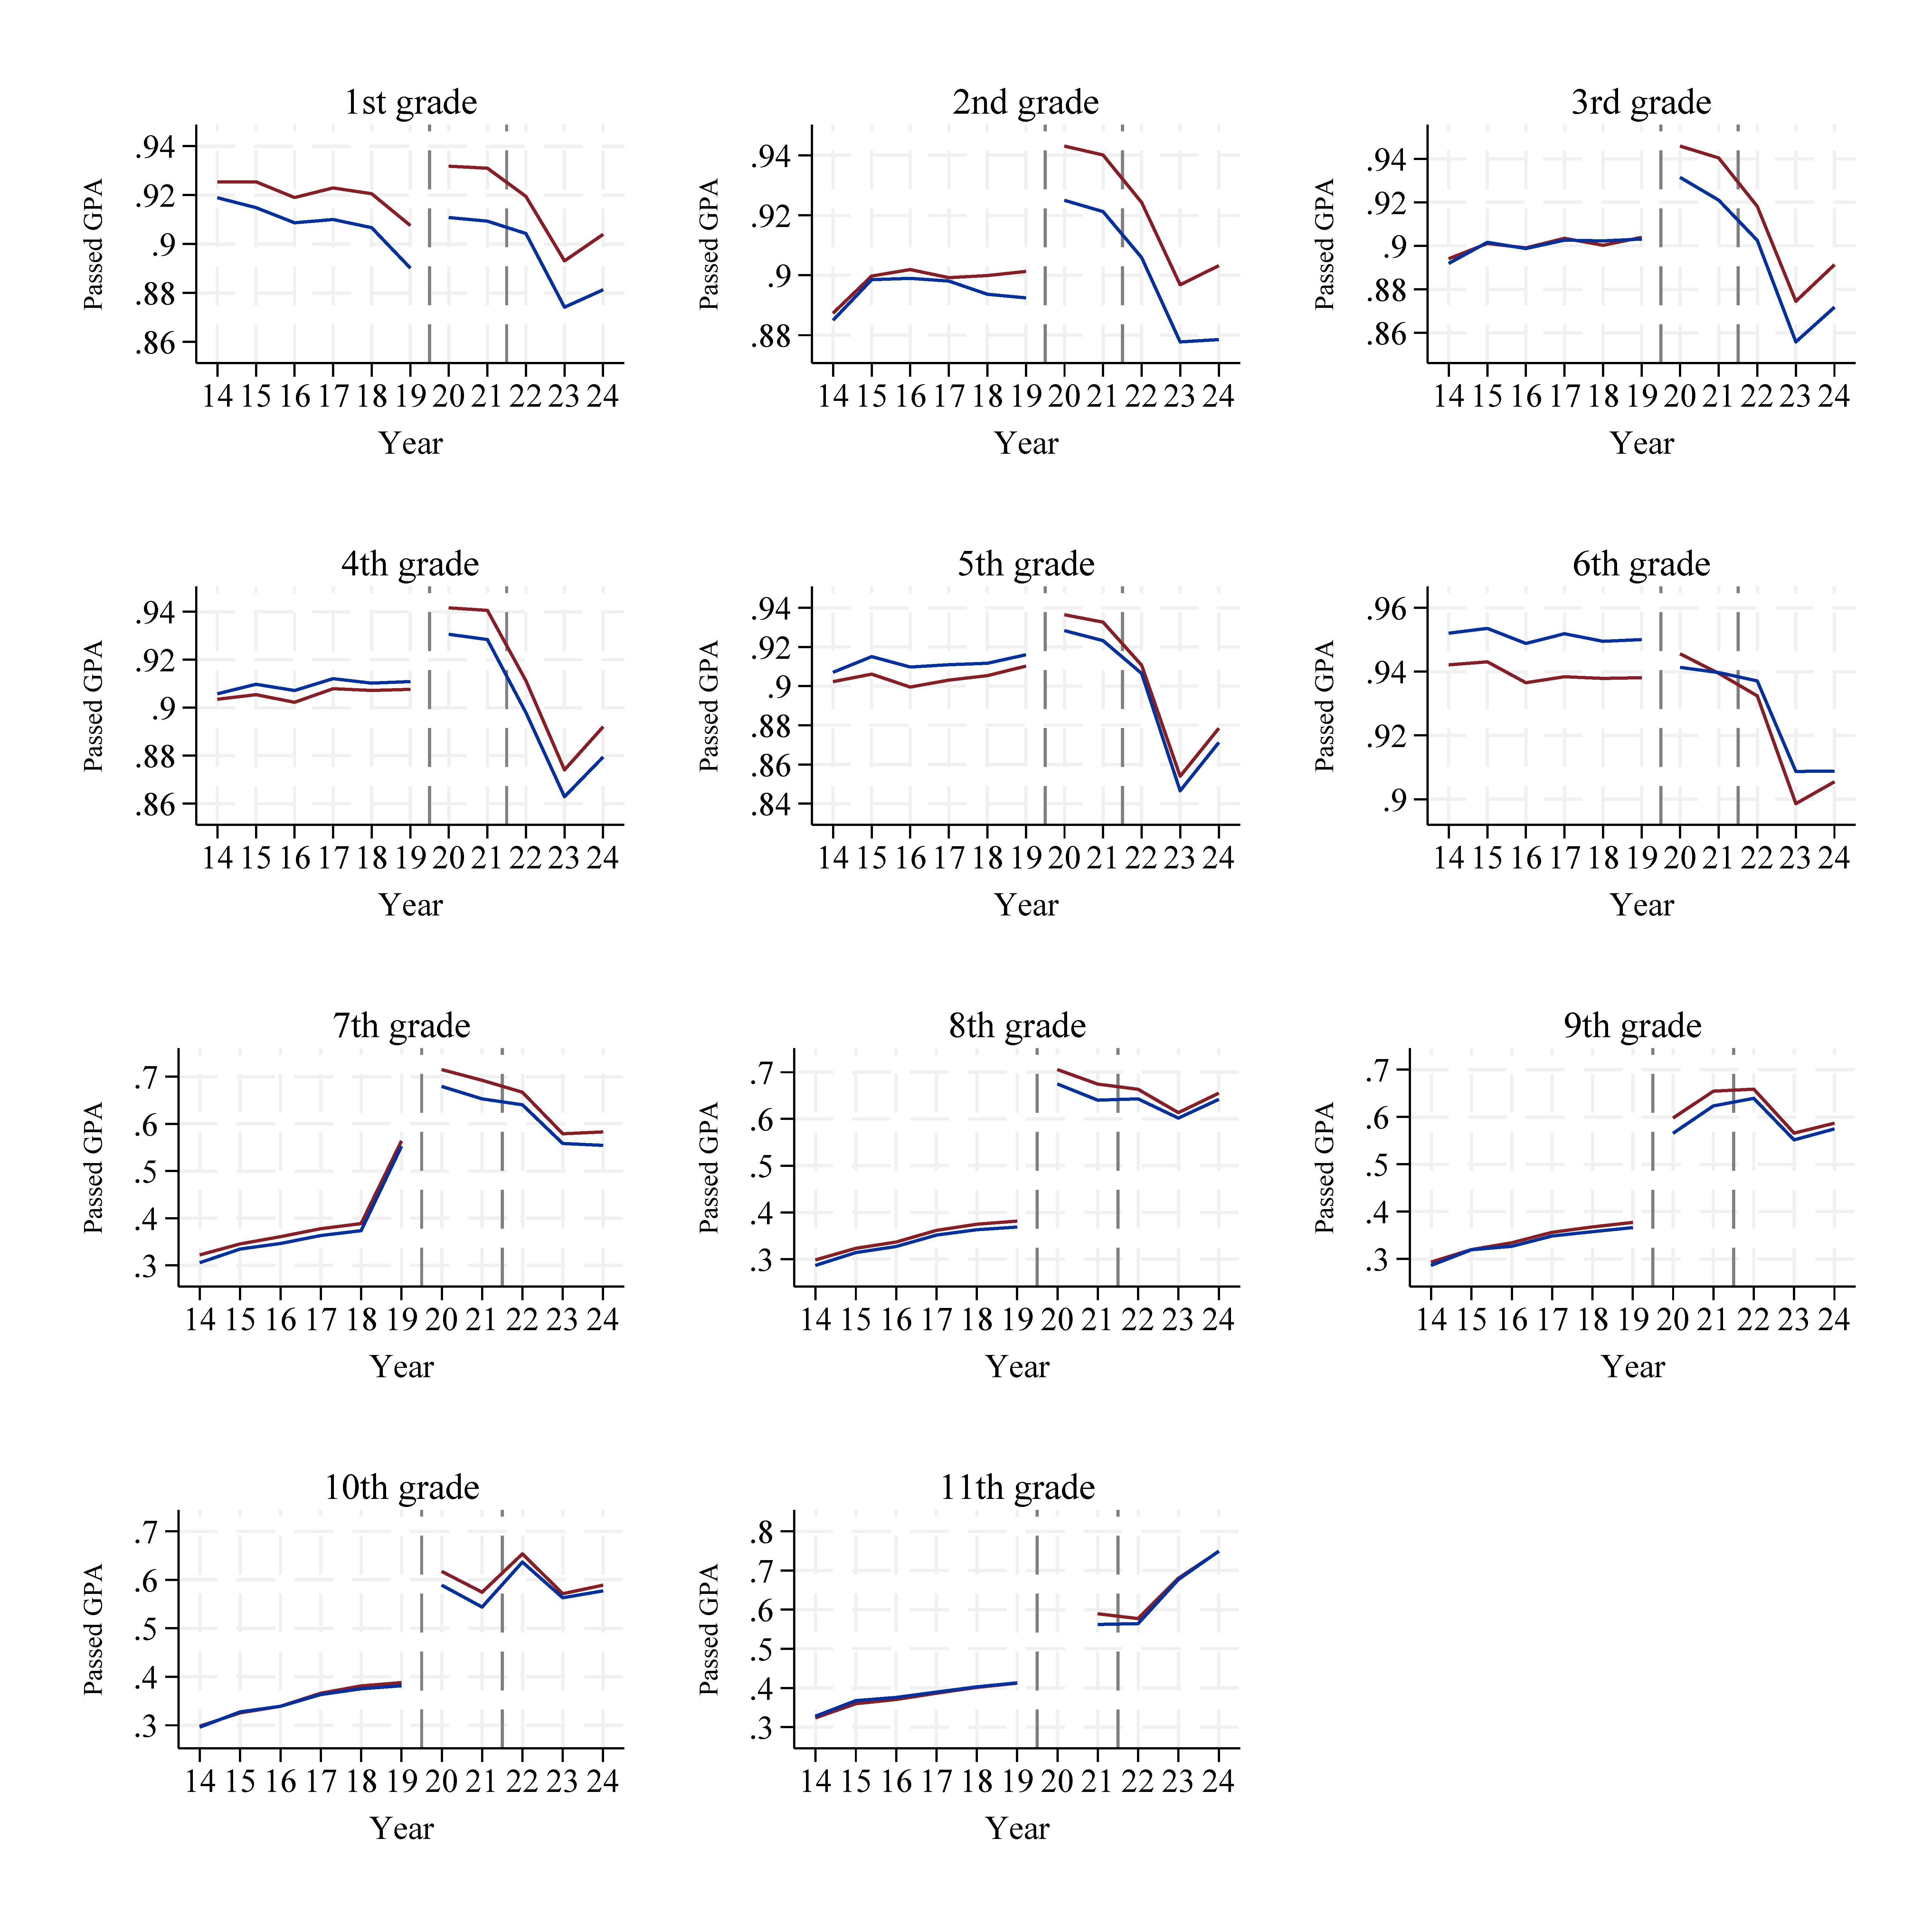
\includegraphics[width=\textwidth]{./FIGURES/Descriptive/raw_grades_pass_math_siblings.pdf}
        \caption{\% of students with an A in Mathematics for each grade 1st-1th}
        \label{fig:trend_pass_grades}
\end{figure}

\begin{figure}[htbp]
         \centering
        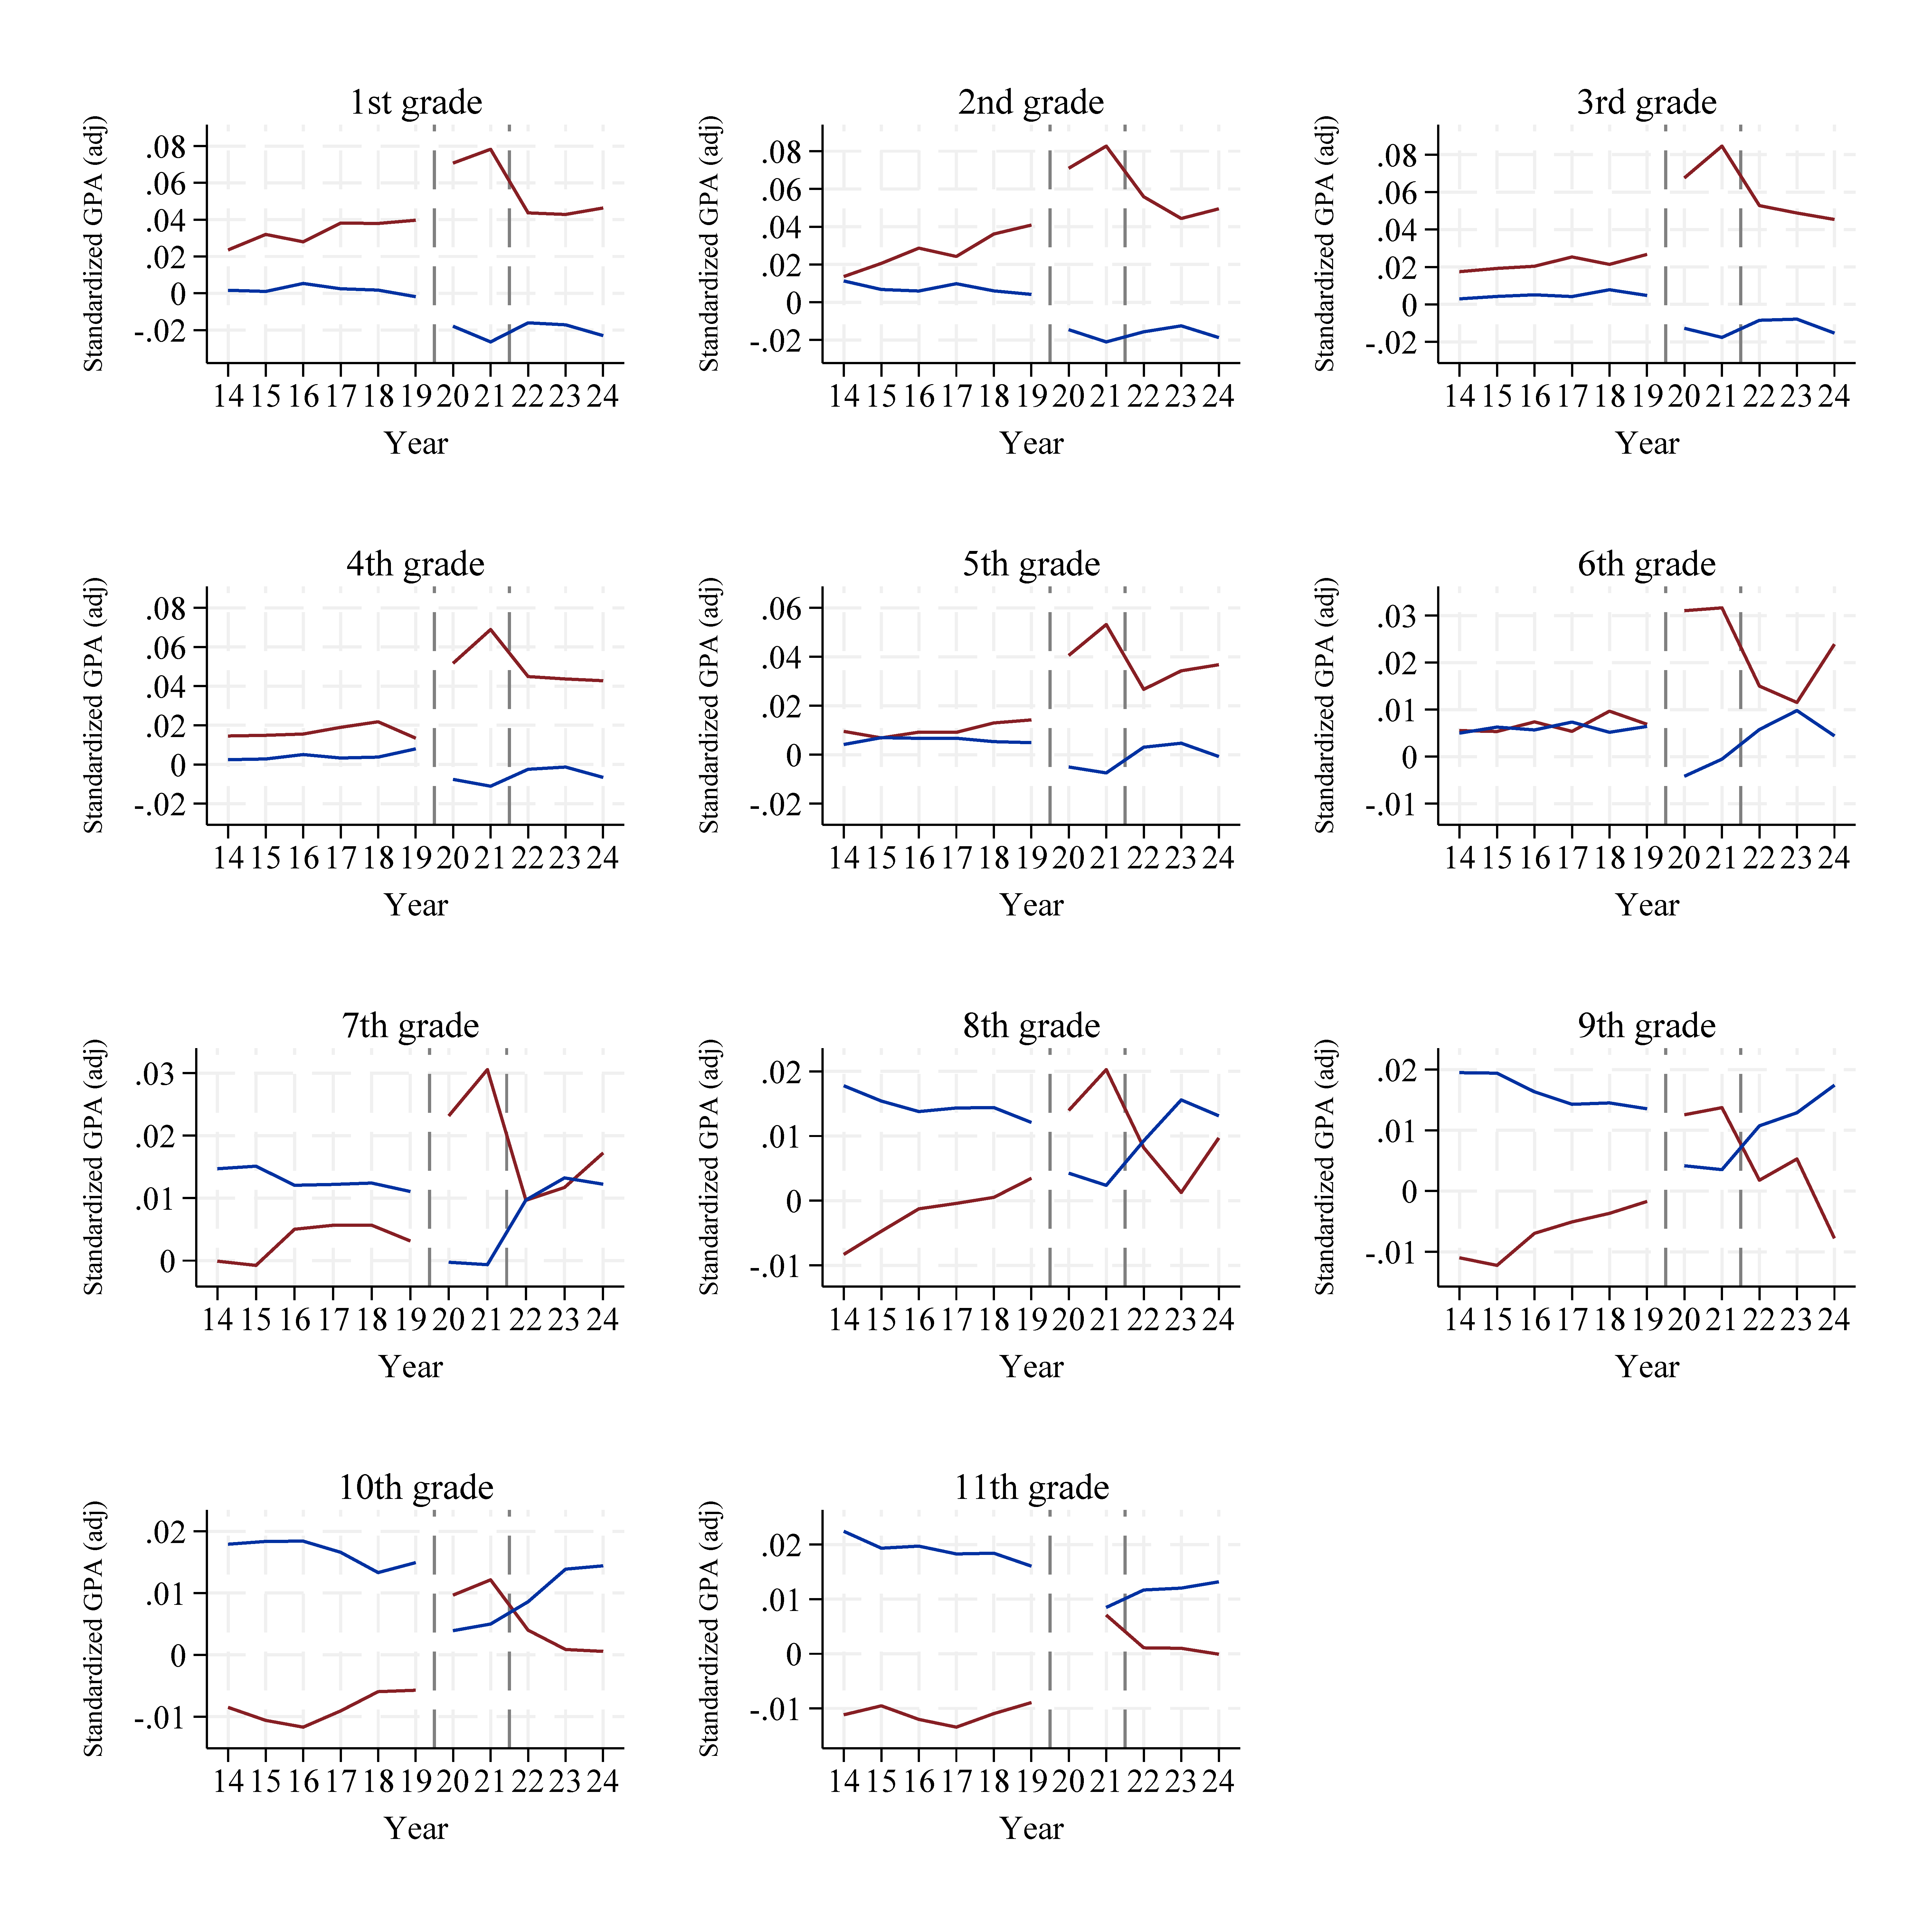
\includegraphics[width=\textwidth]{./FIGURES/Descriptive/raw_grades_std_gpa_m_adj_siblings.pdf}
        \caption{Average GPA standardized within school-grade-year for each grade 1st-1th}
        \label{fig:trend_gpa_grades}
\end{figure}



\begin{figure}[htbp]
    \centering
    
        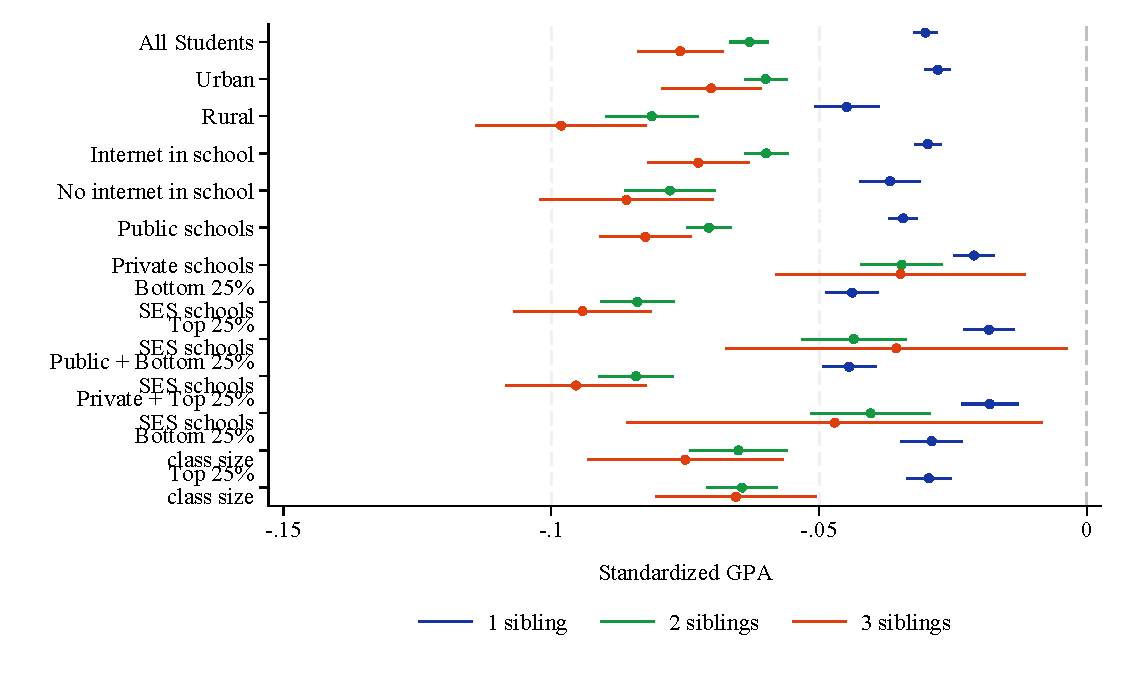
\includegraphics[width=\textwidth]{./FIGURES/TWFE/covid_twfe_A_bysibs_elm_all_gpa_m_adj_Tsiblings_Soldest_4.pdf}
        \caption{Change in gap between children with siblings and only childs}
        \label{fig:fig_appA}

\end{figure}

\begin{figure}[htbp]
    \centering
    
        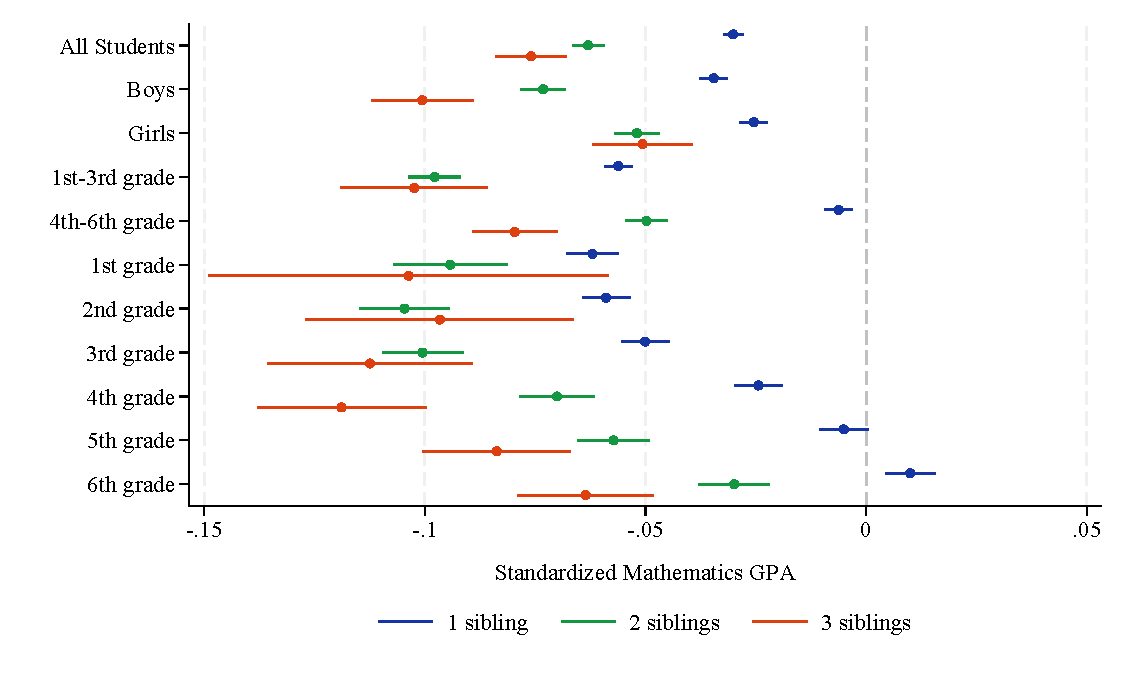
\includegraphics[width=\textwidth]{./FIGURES/TWFE/covid_twfe_B_bysibs_elm_all_gpa_m_adj_Tsiblings_Soldest_4.pdf}
        \caption{Change in gap between children with siblings and only childs}
        \label{fig:fig_appB}

\end{figure}

\begin{figure}[htbp]
    \centering
    
        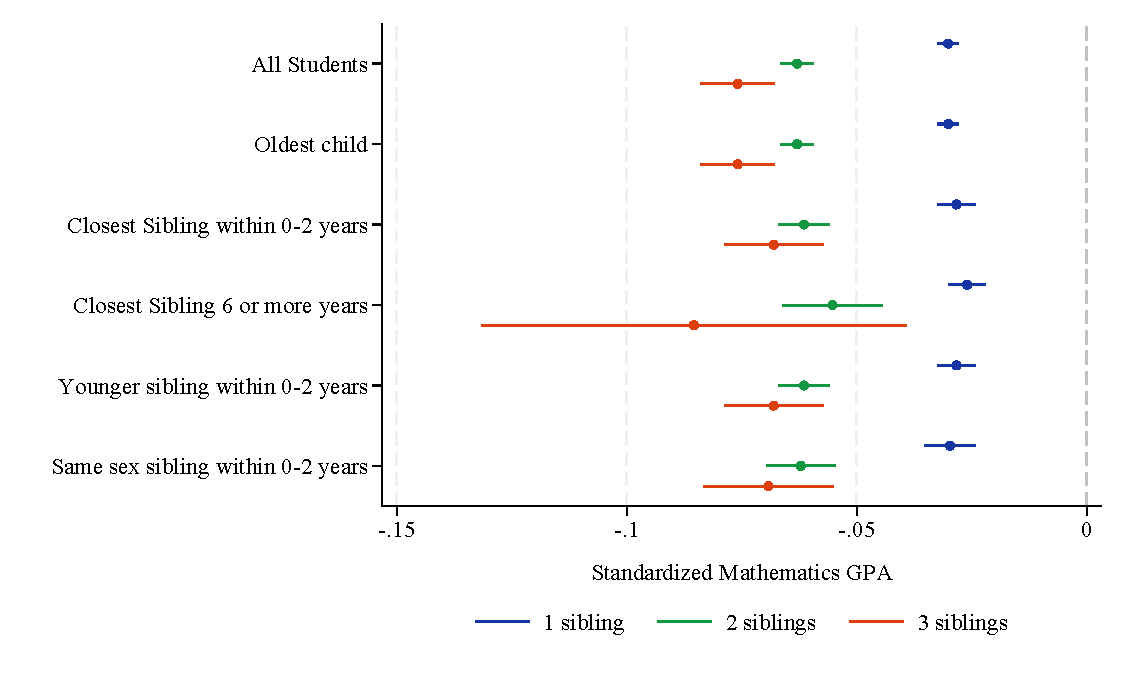
\includegraphics[width=\textwidth]{./FIGURES/TWFE/covid_twfe_C_bysibs_elm_all_gpa_m_adj_Tsiblings_Soldest_4.pdf}
        \caption{Change in gap between children with siblings and only childs}
        \label{fig:fig_appC}

\end{figure}


\begin{figure}[htbp]
    \centering
    
        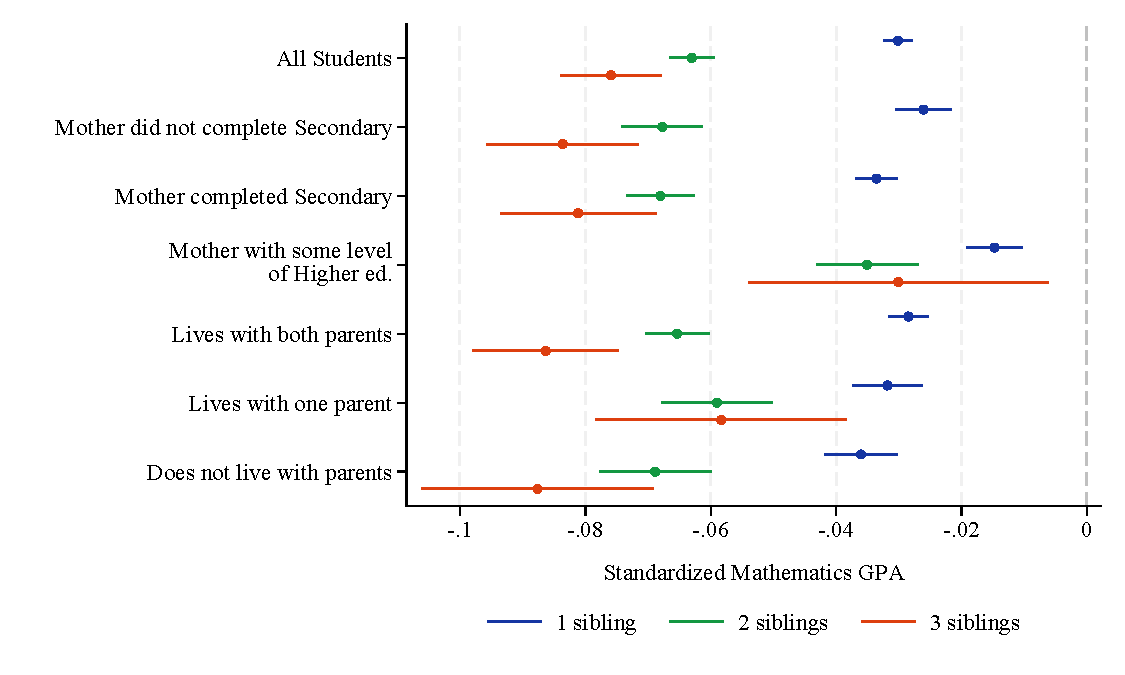
\includegraphics[width=\textwidth]{./FIGURES/TWFE/covid_twfe_D_bysibs_elm_all_gpa_m_adj_Tsiblings_Soldest_4.pdf}
        \caption{Change in gap between children with siblings and only childs}
        \label{fig:fig_appD}

\end{figure}



\end{document}

